
% Default to the notebook output style

    


% Inherit from the specified cell style.




    
\documentclass[11pt]{article}

    
    
    \usepackage[T1]{fontenc}
    % Nicer default font than Computer Modern for most use cases
    \usepackage{palatino}

    % Basic figure setup, for now with no caption control since it's done
    % automatically by Pandoc (which extracts ![](path) syntax from Markdown).
    \usepackage{graphicx}
    % We will generate all images so they have a width \maxwidth. This means
    % that they will get their normal width if they fit onto the page, but
    % are scaled down if they would overflow the margins.
    \makeatletter
    \def\maxwidth{\ifdim\Gin@nat@width>\linewidth\linewidth
    \else\Gin@nat@width\fi}
    \makeatother
    \let\Oldincludegraphics\includegraphics
    % Set max figure width to be 80% of text width, for now hardcoded.
    \renewcommand{\includegraphics}[1]{\Oldincludegraphics[width=.8\maxwidth]{#1}}
    % Ensure that by default, figures have no caption (until we provide a
    % proper Figure object with a Caption API and a way to capture that
    % in the conversion process - todo).
    \usepackage{caption}
    \DeclareCaptionLabelFormat{nolabel}{}
    \captionsetup{labelformat=nolabel}

    \usepackage{adjustbox} % Used to constrain images to a maximum size 
    \usepackage{xcolor} % Allow colors to be defined
    \usepackage{enumerate} % Needed for markdown enumerations to work
    \usepackage{geometry} % Used to adjust the document margins
    \usepackage{amsmath} % Equations
    \usepackage{amssymb} % Equations
    \usepackage{textcomp} % defines textquotesingle
    % Hack from http://tex.stackexchange.com/a/47451/13684:
    \AtBeginDocument{%
        \def\PYZsq{\textquotesingle}% Upright quotes in Pygmentized code
    }
    \usepackage{upquote} % Upright quotes for verbatim code
    \usepackage{eurosym} % defines \euro
    \usepackage[mathletters]{ucs} % Extended unicode (utf-8) support
    \usepackage[utf8x]{inputenc} % Allow utf-8 characters in the tex document
    \usepackage{fancyvrb} % verbatim replacement that allows latex
    \usepackage{grffile} % extends the file name processing of package graphics 
                         % to support a larger range 
    % The hyperref package gives us a pdf with properly built
    % internal navigation ('pdf bookmarks' for the table of contents,
    % internal cross-reference links, web links for URLs, etc.)
    \usepackage{hyperref}
    \usepackage{longtable} % longtable support required by pandoc >1.10
    \usepackage{booktabs}  % table support for pandoc > 1.12.2
    \usepackage[normalem]{ulem} % ulem is needed to support strikethroughs (\sout)
                                % normalem makes italics be italics, not underlines
    

    
    
    % Colors for the hyperref package
    \definecolor{urlcolor}{rgb}{0,.145,.698}
    \definecolor{linkcolor}{rgb}{.71,0.21,0.01}
    \definecolor{citecolor}{rgb}{.12,.54,.11}

    % ANSI colors
    \definecolor{ansi-black}{HTML}{3E424D}
    \definecolor{ansi-black-intense}{HTML}{282C36}
    \definecolor{ansi-red}{HTML}{E75C58}
    \definecolor{ansi-red-intense}{HTML}{B22B31}
    \definecolor{ansi-green}{HTML}{00A250}
    \definecolor{ansi-green-intense}{HTML}{007427}
    \definecolor{ansi-yellow}{HTML}{DDB62B}
    \definecolor{ansi-yellow-intense}{HTML}{B27D12}
    \definecolor{ansi-blue}{HTML}{208FFB}
    \definecolor{ansi-blue-intense}{HTML}{0065CA}
    \definecolor{ansi-magenta}{HTML}{D160C4}
    \definecolor{ansi-magenta-intense}{HTML}{A03196}
    \definecolor{ansi-cyan}{HTML}{60C6C8}
    \definecolor{ansi-cyan-intense}{HTML}{258F8F}
    \definecolor{ansi-white}{HTML}{C5C1B4}
    \definecolor{ansi-white-intense}{HTML}{A1A6B2}

    % commands and environments needed by pandoc snippets
    % extracted from the output of `pandoc -s`
    \providecommand{\tightlist}{%
      \setlength{\itemsep}{0pt}\setlength{\parskip}{0pt}}
    \DefineVerbatimEnvironment{Highlighting}{Verbatim}{commandchars=\\\{\}}
    % Add ',fontsize=\small' for more characters per line
    \newenvironment{Shaded}{}{}
    \newcommand{\KeywordTok}[1]{\textcolor[rgb]{0.00,0.44,0.13}{\textbf{{#1}}}}
    \newcommand{\DataTypeTok}[1]{\textcolor[rgb]{0.56,0.13,0.00}{{#1}}}
    \newcommand{\DecValTok}[1]{\textcolor[rgb]{0.25,0.63,0.44}{{#1}}}
    \newcommand{\BaseNTok}[1]{\textcolor[rgb]{0.25,0.63,0.44}{{#1}}}
    \newcommand{\FloatTok}[1]{\textcolor[rgb]{0.25,0.63,0.44}{{#1}}}
    \newcommand{\CharTok}[1]{\textcolor[rgb]{0.25,0.44,0.63}{{#1}}}
    \newcommand{\StringTok}[1]{\textcolor[rgb]{0.25,0.44,0.63}{{#1}}}
    \newcommand{\CommentTok}[1]{\textcolor[rgb]{0.38,0.63,0.69}{\textit{{#1}}}}
    \newcommand{\OtherTok}[1]{\textcolor[rgb]{0.00,0.44,0.13}{{#1}}}
    \newcommand{\AlertTok}[1]{\textcolor[rgb]{1.00,0.00,0.00}{\textbf{{#1}}}}
    \newcommand{\FunctionTok}[1]{\textcolor[rgb]{0.02,0.16,0.49}{{#1}}}
    \newcommand{\RegionMarkerTok}[1]{{#1}}
    \newcommand{\ErrorTok}[1]{\textcolor[rgb]{1.00,0.00,0.00}{\textbf{{#1}}}}
    \newcommand{\NormalTok}[1]{{#1}}
    
    % Additional commands for more recent versions of Pandoc
    \newcommand{\ConstantTok}[1]{\textcolor[rgb]{0.53,0.00,0.00}{{#1}}}
    \newcommand{\SpecialCharTok}[1]{\textcolor[rgb]{0.25,0.44,0.63}{{#1}}}
    \newcommand{\VerbatimStringTok}[1]{\textcolor[rgb]{0.25,0.44,0.63}{{#1}}}
    \newcommand{\SpecialStringTok}[1]{\textcolor[rgb]{0.73,0.40,0.53}{{#1}}}
    \newcommand{\ImportTok}[1]{{#1}}
    \newcommand{\DocumentationTok}[1]{\textcolor[rgb]{0.73,0.13,0.13}{\textit{{#1}}}}
    \newcommand{\AnnotationTok}[1]{\textcolor[rgb]{0.38,0.63,0.69}{\textbf{\textit{{#1}}}}}
    \newcommand{\CommentVarTok}[1]{\textcolor[rgb]{0.38,0.63,0.69}{\textbf{\textit{{#1}}}}}
    \newcommand{\VariableTok}[1]{\textcolor[rgb]{0.10,0.09,0.49}{{#1}}}
    \newcommand{\ControlFlowTok}[1]{\textcolor[rgb]{0.00,0.44,0.13}{\textbf{{#1}}}}
    \newcommand{\OperatorTok}[1]{\textcolor[rgb]{0.40,0.40,0.40}{{#1}}}
    \newcommand{\BuiltInTok}[1]{{#1}}
    \newcommand{\ExtensionTok}[1]{{#1}}
    \newcommand{\PreprocessorTok}[1]{\textcolor[rgb]{0.74,0.48,0.00}{{#1}}}
    \newcommand{\AttributeTok}[1]{\textcolor[rgb]{0.49,0.56,0.16}{{#1}}}
    \newcommand{\InformationTok}[1]{\textcolor[rgb]{0.38,0.63,0.69}{\textbf{\textit{{#1}}}}}
    \newcommand{\WarningTok}[1]{\textcolor[rgb]{0.38,0.63,0.69}{\textbf{\textit{{#1}}}}}
    
    
    % Define a nice break command that doesn't care if a line doesn't already
    % exist.
    \def\br{\hspace*{\fill} \\* }
    % Math Jax compatability definitions
    \def\gt{>}
    \def\lt{<}
    % Document parameters
    \title{p}
    
    
    

    % Pygments definitions
    
\makeatletter
\def\PY@reset{\let\PY@it=\relax \let\PY@bf=\relax%
    \let\PY@ul=\relax \let\PY@tc=\relax%
    \let\PY@bc=\relax \let\PY@ff=\relax}
\def\PY@tok#1{\csname PY@tok@#1\endcsname}
\def\PY@toks#1+{\ifx\relax#1\empty\else%
    \PY@tok{#1}\expandafter\PY@toks\fi}
\def\PY@do#1{\PY@bc{\PY@tc{\PY@ul{%
    \PY@it{\PY@bf{\PY@ff{#1}}}}}}}
\def\PY#1#2{\PY@reset\PY@toks#1+\relax+\PY@do{#2}}

\expandafter\def\csname PY@tok@gd\endcsname{\def\PY@tc##1{\textcolor[rgb]{0.63,0.00,0.00}{##1}}}
\expandafter\def\csname PY@tok@gu\endcsname{\let\PY@bf=\textbf\def\PY@tc##1{\textcolor[rgb]{0.50,0.00,0.50}{##1}}}
\expandafter\def\csname PY@tok@gt\endcsname{\def\PY@tc##1{\textcolor[rgb]{0.00,0.27,0.87}{##1}}}
\expandafter\def\csname PY@tok@gs\endcsname{\let\PY@bf=\textbf}
\expandafter\def\csname PY@tok@gr\endcsname{\def\PY@tc##1{\textcolor[rgb]{1.00,0.00,0.00}{##1}}}
\expandafter\def\csname PY@tok@cm\endcsname{\let\PY@it=\textit\def\PY@tc##1{\textcolor[rgb]{0.25,0.50,0.50}{##1}}}
\expandafter\def\csname PY@tok@vg\endcsname{\def\PY@tc##1{\textcolor[rgb]{0.10,0.09,0.49}{##1}}}
\expandafter\def\csname PY@tok@vi\endcsname{\def\PY@tc##1{\textcolor[rgb]{0.10,0.09,0.49}{##1}}}
\expandafter\def\csname PY@tok@mh\endcsname{\def\PY@tc##1{\textcolor[rgb]{0.40,0.40,0.40}{##1}}}
\expandafter\def\csname PY@tok@cs\endcsname{\let\PY@it=\textit\def\PY@tc##1{\textcolor[rgb]{0.25,0.50,0.50}{##1}}}
\expandafter\def\csname PY@tok@ge\endcsname{\let\PY@it=\textit}
\expandafter\def\csname PY@tok@vc\endcsname{\def\PY@tc##1{\textcolor[rgb]{0.10,0.09,0.49}{##1}}}
\expandafter\def\csname PY@tok@il\endcsname{\def\PY@tc##1{\textcolor[rgb]{0.40,0.40,0.40}{##1}}}
\expandafter\def\csname PY@tok@go\endcsname{\def\PY@tc##1{\textcolor[rgb]{0.53,0.53,0.53}{##1}}}
\expandafter\def\csname PY@tok@cp\endcsname{\def\PY@tc##1{\textcolor[rgb]{0.74,0.48,0.00}{##1}}}
\expandafter\def\csname PY@tok@gi\endcsname{\def\PY@tc##1{\textcolor[rgb]{0.00,0.63,0.00}{##1}}}
\expandafter\def\csname PY@tok@gh\endcsname{\let\PY@bf=\textbf\def\PY@tc##1{\textcolor[rgb]{0.00,0.00,0.50}{##1}}}
\expandafter\def\csname PY@tok@ni\endcsname{\let\PY@bf=\textbf\def\PY@tc##1{\textcolor[rgb]{0.60,0.60,0.60}{##1}}}
\expandafter\def\csname PY@tok@nl\endcsname{\def\PY@tc##1{\textcolor[rgb]{0.63,0.63,0.00}{##1}}}
\expandafter\def\csname PY@tok@nn\endcsname{\let\PY@bf=\textbf\def\PY@tc##1{\textcolor[rgb]{0.00,0.00,1.00}{##1}}}
\expandafter\def\csname PY@tok@no\endcsname{\def\PY@tc##1{\textcolor[rgb]{0.53,0.00,0.00}{##1}}}
\expandafter\def\csname PY@tok@na\endcsname{\def\PY@tc##1{\textcolor[rgb]{0.49,0.56,0.16}{##1}}}
\expandafter\def\csname PY@tok@nb\endcsname{\def\PY@tc##1{\textcolor[rgb]{0.00,0.50,0.00}{##1}}}
\expandafter\def\csname PY@tok@nc\endcsname{\let\PY@bf=\textbf\def\PY@tc##1{\textcolor[rgb]{0.00,0.00,1.00}{##1}}}
\expandafter\def\csname PY@tok@nd\endcsname{\def\PY@tc##1{\textcolor[rgb]{0.67,0.13,1.00}{##1}}}
\expandafter\def\csname PY@tok@ne\endcsname{\let\PY@bf=\textbf\def\PY@tc##1{\textcolor[rgb]{0.82,0.25,0.23}{##1}}}
\expandafter\def\csname PY@tok@nf\endcsname{\def\PY@tc##1{\textcolor[rgb]{0.00,0.00,1.00}{##1}}}
\expandafter\def\csname PY@tok@si\endcsname{\let\PY@bf=\textbf\def\PY@tc##1{\textcolor[rgb]{0.73,0.40,0.53}{##1}}}
\expandafter\def\csname PY@tok@s2\endcsname{\def\PY@tc##1{\textcolor[rgb]{0.73,0.13,0.13}{##1}}}
\expandafter\def\csname PY@tok@nt\endcsname{\let\PY@bf=\textbf\def\PY@tc##1{\textcolor[rgb]{0.00,0.50,0.00}{##1}}}
\expandafter\def\csname PY@tok@nv\endcsname{\def\PY@tc##1{\textcolor[rgb]{0.10,0.09,0.49}{##1}}}
\expandafter\def\csname PY@tok@s1\endcsname{\def\PY@tc##1{\textcolor[rgb]{0.73,0.13,0.13}{##1}}}
\expandafter\def\csname PY@tok@ch\endcsname{\let\PY@it=\textit\def\PY@tc##1{\textcolor[rgb]{0.25,0.50,0.50}{##1}}}
\expandafter\def\csname PY@tok@m\endcsname{\def\PY@tc##1{\textcolor[rgb]{0.40,0.40,0.40}{##1}}}
\expandafter\def\csname PY@tok@gp\endcsname{\let\PY@bf=\textbf\def\PY@tc##1{\textcolor[rgb]{0.00,0.00,0.50}{##1}}}
\expandafter\def\csname PY@tok@sh\endcsname{\def\PY@tc##1{\textcolor[rgb]{0.73,0.13,0.13}{##1}}}
\expandafter\def\csname PY@tok@ow\endcsname{\let\PY@bf=\textbf\def\PY@tc##1{\textcolor[rgb]{0.67,0.13,1.00}{##1}}}
\expandafter\def\csname PY@tok@sx\endcsname{\def\PY@tc##1{\textcolor[rgb]{0.00,0.50,0.00}{##1}}}
\expandafter\def\csname PY@tok@bp\endcsname{\def\PY@tc##1{\textcolor[rgb]{0.00,0.50,0.00}{##1}}}
\expandafter\def\csname PY@tok@c1\endcsname{\let\PY@it=\textit\def\PY@tc##1{\textcolor[rgb]{0.25,0.50,0.50}{##1}}}
\expandafter\def\csname PY@tok@o\endcsname{\def\PY@tc##1{\textcolor[rgb]{0.40,0.40,0.40}{##1}}}
\expandafter\def\csname PY@tok@kc\endcsname{\let\PY@bf=\textbf\def\PY@tc##1{\textcolor[rgb]{0.00,0.50,0.00}{##1}}}
\expandafter\def\csname PY@tok@c\endcsname{\let\PY@it=\textit\def\PY@tc##1{\textcolor[rgb]{0.25,0.50,0.50}{##1}}}
\expandafter\def\csname PY@tok@mf\endcsname{\def\PY@tc##1{\textcolor[rgb]{0.40,0.40,0.40}{##1}}}
\expandafter\def\csname PY@tok@err\endcsname{\def\PY@bc##1{\setlength{\fboxsep}{0pt}\fcolorbox[rgb]{1.00,0.00,0.00}{1,1,1}{\strut ##1}}}
\expandafter\def\csname PY@tok@mb\endcsname{\def\PY@tc##1{\textcolor[rgb]{0.40,0.40,0.40}{##1}}}
\expandafter\def\csname PY@tok@ss\endcsname{\def\PY@tc##1{\textcolor[rgb]{0.10,0.09,0.49}{##1}}}
\expandafter\def\csname PY@tok@sr\endcsname{\def\PY@tc##1{\textcolor[rgb]{0.73,0.40,0.53}{##1}}}
\expandafter\def\csname PY@tok@mo\endcsname{\def\PY@tc##1{\textcolor[rgb]{0.40,0.40,0.40}{##1}}}
\expandafter\def\csname PY@tok@kd\endcsname{\let\PY@bf=\textbf\def\PY@tc##1{\textcolor[rgb]{0.00,0.50,0.00}{##1}}}
\expandafter\def\csname PY@tok@mi\endcsname{\def\PY@tc##1{\textcolor[rgb]{0.40,0.40,0.40}{##1}}}
\expandafter\def\csname PY@tok@kn\endcsname{\let\PY@bf=\textbf\def\PY@tc##1{\textcolor[rgb]{0.00,0.50,0.00}{##1}}}
\expandafter\def\csname PY@tok@cpf\endcsname{\let\PY@it=\textit\def\PY@tc##1{\textcolor[rgb]{0.25,0.50,0.50}{##1}}}
\expandafter\def\csname PY@tok@kr\endcsname{\let\PY@bf=\textbf\def\PY@tc##1{\textcolor[rgb]{0.00,0.50,0.00}{##1}}}
\expandafter\def\csname PY@tok@s\endcsname{\def\PY@tc##1{\textcolor[rgb]{0.73,0.13,0.13}{##1}}}
\expandafter\def\csname PY@tok@kp\endcsname{\def\PY@tc##1{\textcolor[rgb]{0.00,0.50,0.00}{##1}}}
\expandafter\def\csname PY@tok@w\endcsname{\def\PY@tc##1{\textcolor[rgb]{0.73,0.73,0.73}{##1}}}
\expandafter\def\csname PY@tok@kt\endcsname{\def\PY@tc##1{\textcolor[rgb]{0.69,0.00,0.25}{##1}}}
\expandafter\def\csname PY@tok@sc\endcsname{\def\PY@tc##1{\textcolor[rgb]{0.73,0.13,0.13}{##1}}}
\expandafter\def\csname PY@tok@sb\endcsname{\def\PY@tc##1{\textcolor[rgb]{0.73,0.13,0.13}{##1}}}
\expandafter\def\csname PY@tok@k\endcsname{\let\PY@bf=\textbf\def\PY@tc##1{\textcolor[rgb]{0.00,0.50,0.00}{##1}}}
\expandafter\def\csname PY@tok@se\endcsname{\let\PY@bf=\textbf\def\PY@tc##1{\textcolor[rgb]{0.73,0.40,0.13}{##1}}}
\expandafter\def\csname PY@tok@sd\endcsname{\let\PY@it=\textit\def\PY@tc##1{\textcolor[rgb]{0.73,0.13,0.13}{##1}}}

\def\PYZbs{\char`\\}
\def\PYZus{\char`\_}
\def\PYZob{\char`\{}
\def\PYZcb{\char`\}}
\def\PYZca{\char`\^}
\def\PYZam{\char`\&}
\def\PYZlt{\char`\<}
\def\PYZgt{\char`\>}
\def\PYZsh{\char`\#}
\def\PYZpc{\char`\%}
\def\PYZdl{\char`\$}
\def\PYZhy{\char`\-}
\def\PYZsq{\char`\'}
\def\PYZdq{\char`\"}
\def\PYZti{\char`\~}
% for compatibility with earlier versions
\def\PYZat{@}
\def\PYZlb{[}
\def\PYZrb{]}
\makeatother


    % Exact colors from NB
    \definecolor{incolor}{rgb}{0.0, 0.0, 0.5}
    \definecolor{outcolor}{rgb}{0.545, 0.0, 0.0}
    
    \usepackage[framemethod=tikz]{mdframed}



    
    % Prevent overflowing lines due to hard-to-break entities
    \sloppy 
    % Setup hyperref package
    \hypersetup{
      breaklinks=true,  % so long urls are correctly broken across lines
      colorlinks=true,
      urlcolor=urlcolor,
      linkcolor=linkcolor,
      citecolor=citecolor,
      }
    % Slightly bigger margins than the latex defaults
    
    \geometry{verbose,tmargin=1in,bmargin=1in,lmargin=1in,rmargin=1in}
    
    

    \begin{document}
    
    
    \maketitle
    
    

    
    \section{Table of Contents}\label{table-of-contents}

{1~~}Resumen teórico

{1.1~~}Explicación intuitiva

{1.2~~}Parametrización

{1.3~~}Definición formal del problema

{1.4~~}Matriz de confusión

{2~~}Ejecución práctica

{2.1~~}Estudio de iris.arff ignorando la clase

{2.1.1~~}Entrenamiento con todos los datos

{2.1.2~~}Entrenamiento con 2/3 de los datos

{2.1.3~~}Comparación de entrenamiento total vs.~2/3

{2.1.3.1~~}Análisis de centroides

{2.1.4~~}Análisis y representación de regiones

{2.1.4.1~~}Representación de regiones por pares de atributos enfrentados

{2.1.4.2~~}Representación de regiones frente a número de instancia

{2.2~~}Estudio de iris.arff utilizando la clase

{2.2.1~~}Representación de clusters, instancias y aciertos

{2.2.2~~}Comentario de las agrupaciones obtenidas

{2.2.3~~}Matrices de confusión obtenidas

{2.3~~}Experimentos basados en cambiar la semilla

{2.4~~}Experimentos basados en descartar atributos

{2.4.1~~}Descartamos `sepal length'

{2.4.2~~}Descartamos `sepal width'

{2.4.3~~}Descartamos `petal length'

{2.4.4~~}Descartamos `petal width'

{2.4.5~~}Experimento con ``petal length'' y ``petal width''

{2.4.6~~}Conlusión

{2.5~~}Experimentos basados en cambiar el número de grupos k

{3~~}Conclusiones

{4~~}Referencias

    \section{Resumen teórico}\label{resumen-teuxf3rico}

El algoritmo de \textbf{k-medias} (en inglés k-means) es el algoritmo de
clustering por vecindad más popular actualmente {[}3{]}.

K-medias produce particiones de los datos, es decir, una vez aplicado
los datos no pueden pertenecer a 2 categorías como por ejemplo en los
algoritmos que generan particiones jerárquicas.

\subsection{Explicación intuitiva}\label{explicaciuxf3n-intuitiva}

K-medias parte de un estado inicial con una serie de patrones sin
etiquetar y unos vectores cuyos valores han sido inicializados
aleatoriamente que representarán cada una de las k categorías en las que
queremos clasificar los patrones{[}2{]}. Cada vez que mostramos un nuevo
patrón al algoritmo, es comparado con todos los vectores existentes
(denominados \textbf{centroides}) y se etiquetará con la clase del
centroide que esté a menor distancia del patrón.

Por tanto ya hemos definido los parametros necesarios para ejecutar el
algorimo k-medias:

\begin{itemize}
\tightlist
\item
  Un conjunto de patrones de entrenamiento
\item
  Un número de grupos k en el que queremos particionar los datos
\item
  Una métrica para medir la distancia entre los patrones (normalmente se
  utiliza la distancia euclidea)
\end{itemize}

\begin{figure}
\centering
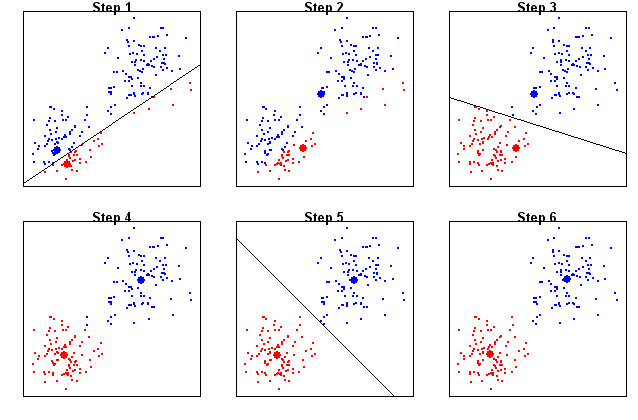
\includegraphics{k_means.png}
\caption{k-means}
\end{figure}

\emph{Figura 1: Ejemplo gráfico de entrenamiento del algoritmo K-medias
para 2 clases}

El proceso de entrenamiento se reduce a conseguir que los centroides
sean puntos significativos para cada cluster k, esto se consigue de la
siguiente forma:

\begin{enumerate}
\def\labelenumi{\arabic{enumi}.}
\tightlist
\item
  Para cada patrón del conjutno de entrenamiento, determinar el
  centroide más cercano y añadir el patrón a la lista de patrones del
  centroide
\item
  Una vez asignados todos los patrones a su centroide más cercano,
  volver a calcular los valores de los centroides a partir de los
  patrones que pertenecen a su lista
\item
  Repetir este proceso hasta que los centroides convergan (se
  estabilicen y no se muevan)
\end{enumerate}

Mediante este proceso dividimos los patrones de entrenamiento en k
regiones, cada una con su prototipo en el centro. Aunque el proceso de
entrenamiento puede ser largo, \textbf{una vez entrenado el sitema
clasificar patrones es inmediato}, ya que sólo hay que calcular la
distancia entre el patrón y los centroides y asignar el patrón al
cluster del centroide más cercano.

En la siguiente figura podemos ver la curva que sigue el movimiento de
los tres centroides de un ejemplo de entrenamiento de k-means con 3
regiones:

\begin{figure}
\centering
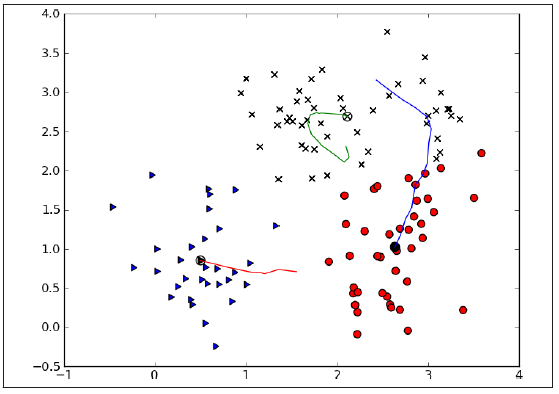
\includegraphics{image-4.png}
\caption{k-means}
\end{figure}

\emph{Figura 2: Ejemplo de la evolución de los centroides}

Dado que \textbf{en la mayoría de casos en los que se utilizaría este
algoritmo desconocemos la clase de los patrones}, es difícil establecer
métricas para medir la bondad del modelo obtenido. Más tarde veremos el
concepto de matriz de confusión.

\subsection{Parametrización}\label{parametrizaciuxf3n}

El primer parámetro significativo en el algoritmo k-means es el número
de regiones que queremos que se generen.

Si estamos en un problema supervisado, en dónde conocemos de antemano el
número de clases, lo más normal es generar tantas regiones como clases
haya. Si no se conoce de antemano el número de clases posibles, entonces
habrá que probar con distintos valores de K para determinar qué numero
de regiones dividen el problema de forma apropiada para cada caso de
uso.

En relación a la posición inicial de los centroides se suelen seguir
distintos métodos:

\begin{itemize}
\tightlist
\item
  se pueden generar de forma aleatoria
\item
  o se pueden elegir k patrones del conjunto de datos y utilizar estos
  mismos patrones con centroides iniciales
\item
  o se pueden asignar aleatorimente los patrones a k grupos y calcular
  los centroides de cada grupo (ya en el paso 2 del algoritmo)
\end{itemize}

\subsection{Definición formal del
problema}\label{definiciuxf3n-formal-del-problema}

El algoritmo k-means tiene por objeto resolver la tarea de clustering
(agrupamiento) que consiste en, dado un conjunto de datos, generar una
serie de grupos de manera que los individuos perteneciente a cada grupo
encontrado presenten características similares entre sí y, a su vez,
distintas a la de los individuos pertenecientes al resto de grupos.

Formalmente, dado un conjunto de observaciones \((x_1, x_2, ..., x_n)\),
donde cada observación es un vertor real de dimensión \(d\), el
agrupamiento con el algoritmo k-medias intenta particionar las \(n\)
observacionesen \(k (\le n)\) en \(k\) conjuntos
\(S = \{S_1, S_2, ..., S_k\}\) de modo que se minimice la suma de
distancias al cuadrado dentro de cada grupo (cluster), es decir, la
varianza.

\[\underset{S}{\mathrm{argmin}} \sum_{i=1}^{k} \sum_{x \in S_i} \|x -\mu_i\|^2\]

siendo \(\mu_i\) la media de los puntos del conjunto \(S_i\) (el
centroide).

\subsection{Matriz de confusión}\label{matriz-de-confusiuxf3n}

Si pensamos en k-medias como un clasificador, en el sentido de que
patrones similares son etiquetados en la misma clase, un método sencillo
para entender como se comporta el clasificador es utilizar una
\textbf{matriz de confusión}{[}1{]}.

En una matriz de confusión la clase dada por el modelo está escrita en
las columnas mientras que la etiqueta real esta escrita en las filas.
Cada celda de la matriz cuenta cuantas instancias de la clase real han
sido clasificadas en cada clase por lo que con esta matriz podemos ver
de forma sencilla como de a menudo una clase es incorrectamente
clasificada.

Una clasificación perfecta produciría una matriz con todo ceros excepto
la diagonal (suponiendo que los clusters están ordenados en la matriz
apropiadamente), mientras que una mala clasificación produciría valores
elevados fuera de la diagonal.

\begin{figure}
\centering
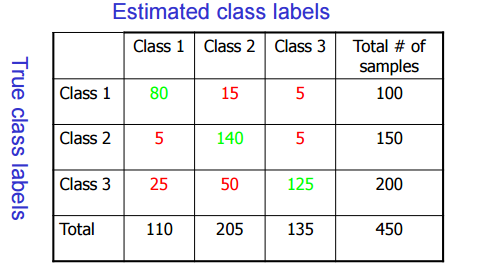
\includegraphics{confusion_matrix.PNG}
\caption{confusion-matrix}
\end{figure}

\emph{Figura 2: Ejemplo de matriz de confusión}

Nótese que en el caso de k-means los nombres de las columnas tendrán que
ser los distintos grupos (clusters) generados por el algoritmo y que
potencialmente tendrán que verse sometidos a reordenación apropiada para
que la regla de la diagonal tenga sentido.

    \section{Ejecución práctica}\label{ejecuciuxf3n-pruxe1ctica}

\subsection{Estudio de iris.arff ignorando la
clase}\label{estudio-de-iris.arff-ignorando-la-clase}

Cargamos el conjunto de datos:

    \begingroup
\fontsize{8pt}{10pt}
\begin{mdframed}[hidealllines=true,backgroundcolor=blue!5]

\begin{Verbatim}[commandchars=\\\{\}]
\PY{k+kn}{from} \PY{n+nn}{sklearn} \PY{k+kn}{import} \PY{n}{datasets}

\PY{n}{iris} \PY{o}{=} \PY{n}{datasets}\PY{o}{.}\PY{n}{load\PYZus{}iris}\PY{p}{(}\PY{p}{)} 
\end{Verbatim}

\end{mdframed}
\endgroup

    \subsubsection{Entrenamiento con todos los
datos}\label{entrenamiento-con-todos-los-datos}

Entrenamos el modelo k-means en todos los datos con todos los parámetros
por defecto, excepto el número de clusters que queremos que sea 3, pues
sabemos que es el número de clases del conjunto iris. Nótese que
iris.data no contiene la clase, por lo que no se está haciendo uso de la
misma en este ejercicio.

A continuación podemos ver los centroides de los clusters que se
obtienen entrenando en todos los datos:

    \begingroup
\fontsize{8pt}{10pt}
\begin{mdframed}[hidealllines=true,backgroundcolor=blue!5]

\begin{Verbatim}[commandchars=\\\{\}]
\PY{k+kn}{from} \PY{n+nn}{sklearn.cluster} \PY{k+kn}{import} \PY{n}{KMeans}
\PY{k+kn}{from} \PY{n+nn}{helper} \PY{k+kn}{import} \PY{n}{get\PYZus{}if\PYZus{}already\PYZus{}done}\PY{p}{,} \PY{n}{save\PYZus{}object}


\PY{k}{def} \PY{n+nf}{run\PYZus{}all\PYZus{}data}\PY{p}{(}\PY{p}{)}\PY{p}{:}
    \PY{n}{name} \PY{o}{=} \PY{l+s+s1}{\PYZsq{}}\PY{l+s+s1}{data/all\PYZus{}model.pkl}\PY{l+s+s1}{\PYZsq{}}
    \PY{k}{if} \PY{n}{get\PYZus{}if\PYZus{}already\PYZus{}done}\PY{p}{(}\PY{n}{name}\PY{p}{)}\PY{p}{:}
        \PY{k}{return} \PY{n}{get\PYZus{}if\PYZus{}already\PYZus{}done}\PY{p}{(}\PY{n}{name}\PY{p}{)}

    \PY{n}{model} \PY{o}{=} \PY{n}{KMeans}\PY{p}{(}\PY{n}{n\PYZus{}clusters}\PY{o}{=}\PY{l+m+mi}{3}\PY{p}{)}\PY{o}{.}\PY{n}{fit}\PY{p}{(}\PY{n}{iris}\PY{o}{.}\PY{n}{data}\PY{p}{)}
    \PY{n}{save\PYZus{}object}\PY{p}{(}\PY{n}{name}\PY{p}{,} \PY{n}{model}\PY{p}{)}
    \PY{k}{return} \PY{n}{model}


\PY{n}{all\PYZus{}model} \PY{o}{=} \PY{n}{run\PYZus{}all\PYZus{}data}\PY{p}{(}\PY{p}{)}
\PY{n}{all\PYZus{}data\PYZus{}centroids} \PY{o}{=} \PY{n}{all\PYZus{}model}\PY{o}{.}\PY{n}{cluster\PYZus{}centers\PYZus{}}
\PY{k}{print} \PY{l+s+s2}{\PYZdq{}}\PY{l+s+s2}{Centroides con todos los datos:}\PY{l+s+s2}{\PYZdq{}}
\PY{k}{print} \PY{n}{all\PYZus{}data\PYZus{}centroids}\PY{o}{.}\PY{n}{round}\PY{p}{(}\PY{l+m+mi}{3}\PY{p}{)} 
\end{Verbatim}

\end{mdframed}
\endgroup

    \begin{Verbatim}[commandchars=\\\{\}]
Centroides con todos los datos:
[[ 5.902  2.748  4.394  1.434]
 [ 5.006  3.418  1.464  0.244]
 [ 6.85   3.074  5.742  2.071]]

    \end{Verbatim}

    \subsubsection{Entrenamiento con 2/3 de los
datos}\label{entrenamiento-con-23-de-los-datos}

Cogemos dos tercios de los datos para entrenar y repetimos el proceso
anterior. \textbf{Nótese que la selección de los datos la realizo con
estratificación} (mantenemos la proporción de las distintas clases en la
muestra y en la población), cosa que influirá en que los resultados
difieran en menor medida que si no se utilizara estratificación.

Vemos los centroides resultantes:

    \begingroup
\fontsize{8pt}{10pt}
\begin{mdframed}[hidealllines=true,backgroundcolor=blue!5]

\begin{Verbatim}[commandchars=\\\{\}]
\PY{k+kn}{from} \PY{n+nn}{sklearn.model\PYZus{}selection} \PY{k+kn}{import} \PY{n}{train\PYZus{}test\PYZus{}split}


\PY{k}{def} \PY{n+nf}{run\PYZus{}partial\PYZus{}data}\PY{p}{(}\PY{p}{)}\PY{p}{:}
    \PY{n}{data} \PY{o}{=} \PY{l+s+s1}{\PYZsq{}}\PY{l+s+s1}{data/partial\PYZus{}data.pkl}\PY{l+s+s1}{\PYZsq{}}
    \PY{n}{name} \PY{o}{=} \PY{l+s+s1}{\PYZsq{}}\PY{l+s+s1}{data/partial\PYZus{}model.pkl}\PY{l+s+s1}{\PYZsq{}}
    \PY{k}{if} \PY{n}{get\PYZus{}if\PYZus{}already\PYZus{}done}\PY{p}{(}\PY{n}{data}\PY{p}{)} \PY{o+ow}{and} \PY{n}{get\PYZus{}if\PYZus{}already\PYZus{}done}\PY{p}{(}\PY{n}{name}\PY{p}{)}\PY{p}{:}
        \PY{k}{return} \PY{n}{get\PYZus{}if\PYZus{}already\PYZus{}done}\PY{p}{(}\PY{n}{name}\PY{p}{)}

    \PY{n}{X\PYZus{}train}\PY{p}{,} \PY{n}{X\PYZus{}test}\PY{p}{,} \PY{n}{y\PYZus{}train}\PY{p}{,} \PY{n}{y\PYZus{}test} \PY{o}{=} \PY{n}{train\PYZus{}test\PYZus{}split}\PY{p}{(}
        \PY{n}{iris}\PY{o}{.}\PY{n}{data}\PY{p}{,} \PY{n}{iris}\PY{o}{.}\PY{n}{target}\PY{p}{,} \PY{n}{test\PYZus{}size}\PY{o}{=}\PY{l+m+mf}{0.33}\PY{p}{,} \PY{n}{stratify}\PY{o}{=}\PY{n}{iris}\PY{o}{.}\PY{n}{target}\PY{p}{)}
    \PY{n}{X\PYZus{}train} \PY{o}{=} \PY{n}{np}\PY{o}{.}\PY{n}{array}\PY{p}{(}\PY{p}{[}\PY{n}{x} \PY{k}{for} \PY{p}{(}\PY{n}{y}\PY{p}{,}\PY{n}{x}\PY{p}{)} \PY{o+ow}{in} 
                        \PY{n+nb}{sorted}\PY{p}{(}\PY{n+nb}{zip}\PY{p}{(}\PY{n}{y\PYZus{}train}\PY{o}{.}\PY{n}{tolist}\PY{p}{(}\PY{p}{)}\PY{p}{,}\PY{n}{X\PYZus{}train}\PY{o}{.}\PY{n}{tolist}\PY{p}{(}\PY{p}{)}\PY{p}{)}\PY{p}{)}\PY{p}{]}\PY{p}{)}
    \PY{n}{y\PYZus{}train} \PY{o}{=} \PY{n}{np}\PY{o}{.}\PY{n}{array}\PY{p}{(}\PY{n+nb}{sorted}\PY{p}{(}\PY{n}{y\PYZus{}train}\PY{p}{)}\PY{p}{)}
    \PY{n}{save\PYZus{}object}\PY{p}{(}\PY{n}{data}\PY{p}{,} \PY{p}{[}\PY{n}{X\PYZus{}train}\PY{p}{,} \PY{n}{X\PYZus{}test}\PY{p}{,} \PY{n}{y\PYZus{}train}\PY{p}{,} \PY{n}{y\PYZus{}test}\PY{p}{]}\PY{p}{)}
    \PY{n}{model} \PY{o}{=} \PY{n}{KMeans}\PY{p}{(}\PY{n}{n\PYZus{}clusters}\PY{o}{=}\PY{l+m+mi}{3}\PY{p}{)}\PY{o}{.}\PY{n}{fit}\PY{p}{(}\PY{n}{X\PYZus{}train}\PY{p}{)}
    \PY{n}{save\PYZus{}object}\PY{p}{(}\PY{n}{name}\PY{p}{,} \PY{n}{model}\PY{p}{)}
    \PY{k}{return} \PY{n}{model}


\PY{n}{partial\PYZus{}model} \PY{o}{=} \PY{n}{run\PYZus{}partial\PYZus{}data}\PY{p}{(}\PY{p}{)}
\PY{n}{partial\PYZus{}data} \PY{o}{=} \PY{n}{get\PYZus{}if\PYZus{}already\PYZus{}done}\PY{p}{(}\PY{l+s+s1}{\PYZsq{}}\PY{l+s+s1}{data/partial\PYZus{}data.pkl}\PY{l+s+s1}{\PYZsq{}}\PY{p}{)}
\PY{n}{partial\PYZus{}data\PYZus{}centroids} \PY{o}{=} \PY{n}{partial\PYZus{}model}\PY{o}{.}\PY{n}{cluster\PYZus{}centers\PYZus{}}
\PY{k}{print} \PY{l+s+s2}{\PYZdq{}}\PY{l+s+s2}{Centroides con 2/3 de los datos:}\PY{l+s+s2}{\PYZdq{}}
\PY{k}{print} \PY{n}{partial\PYZus{}data\PYZus{}centroids}\PY{o}{.}\PY{n}{round}\PY{p}{(}\PY{l+m+mi}{3}\PY{p}{)} 
\end{Verbatim}

\end{mdframed}
\endgroup

    \begin{Verbatim}[commandchars=\\\{\}]
Centroides con 2/3 de los datos:
[[ 5.937  2.732  4.407  1.407]
 [ 4.973  3.309  1.491  0.255]
 [ 6.915  3.088  5.731  2.073]]

    \end{Verbatim}

    \textbf{Nota importante: obsérvese que el conjunto de 2/3 de los datos,
después de la estratificación, lo hemos ordenado según el valor de la
clase. Esto, como explicaré más tarde en la sección de representación de
regiones, hará que la interpretación de los resultados en las
comparaciones sea mucho más clara.}

    \subsubsection{Comparación de entrenamiento total
vs.~2/3}\label{comparaciuxf3n-de-entrenamiento-total-vs.23}

Primero vamos a representar en una tabla los centroides obtenidos en
cada caso:

    \begingroup
\fontsize{8pt}{10pt}
\begin{mdframed}[hidealllines=true,backgroundcolor=blue!5]

\begin{Verbatim}[commandchars=\\\{\}]
\PY{k+kn}{import} \PY{n+nn}{numpy} \PY{k+kn}{as} \PY{n+nn}{np}
\PY{k+kn}{import} \PY{n+nn}{pandas} \PY{k+kn}{as} \PY{n+nn}{pd}
\PY{n}{pd}\PY{o}{.}\PY{n}{set\PYZus{}option}\PY{p}{(}\PY{l+s+s1}{\PYZsq{}}\PY{l+s+s1}{display.notebook\PYZus{}repr\PYZus{}html}\PY{l+s+s1}{\PYZsq{}}\PY{p}{,} \PY{n+nb+bp}{True}\PY{p}{)}


\PY{k}{def} \PY{n+nf}{\PYZus{}repr\PYZus{}latex\PYZus{}}\PY{p}{(}\PY{n+nb+bp}{self}\PY{p}{)}\PY{p}{:}
    \PY{k}{return} \PY{n+nb+bp}{self}\PY{o}{.}\PY{n}{to\PYZus{}latex}\PY{p}{(}\PY{p}{)}


\PY{n}{pd}\PY{o}{.}\PY{n}{DataFrame}\PY{o}{.}\PY{n}{\PYZus{}repr\PYZus{}latex\PYZus{}} \PY{o}{=} \PY{n}{\PYZus{}repr\PYZus{}latex\PYZus{}}

\PY{n}{dtc\PYZus{}df} \PY{o}{=} \PY{n}{pd}\PY{o}{.}\PY{n}{DataFrame}\PY{p}{(}\PY{n}{data}\PY{o}{=}\PY{n}{np}\PY{o}{.}\PY{n}{append}\PY{p}{(}\PY{n}{all\PYZus{}data\PYZus{}centroids}\PY{p}{,}\PY{n}{partial\PYZus{}data\PYZus{}centroids}\PY{p}{,}\PY{n}{axis}\PY{o}{=}\PY{l+m+mi}{0}\PY{p}{)}\PY{p}{,}
                      \PY{n}{columns}\PY{o}{=}\PY{n}{iris}\PY{o}{.}\PY{n}{feature\PYZus{}names}\PY{p}{,}
                      \PY{n}{index}\PY{o}{=}\PY{p}{[}\PY{l+s+s1}{\PYZsq{}}\PY{l+s+s1}{All data centroid }\PY{l+s+s1}{\PYZsq{}} \PY{o}{+} \PY{n+nb}{str}\PY{p}{(}\PY{n}{i}\PY{p}{)} \PY{k}{for} \PY{n}{i} \PY{o+ow}{in} \PY{n+nb}{range}\PY{p}{(}\PY{l+m+mi}{3}\PY{p}{)}\PY{p}{]} \PY{o}{+} \PYZbs{}
                            \PY{p}{[}\PY{l+s+s1}{\PYZsq{}}\PY{l+s+s1}{2/3 data centroid }\PY{l+s+s1}{\PYZsq{}} \PY{o}{+} \PY{n+nb}{str}\PY{p}{(}\PY{n}{i}\PY{p}{)} \PY{k}{for} \PY{n}{i} \PY{o+ow}{in} \PY{n+nb}{range}\PY{p}{(}\PY{l+m+mi}{3}\PY{p}{)}\PY{p}{]} \PY{p}{)}
\PY{n}{dtc\PYZus{}df}\PY{o}{.}\PY{n}{round}\PY{p}{(}\PY{l+m+mi}{4}\PY{p}{)} 
\end{Verbatim}

\end{mdframed}
\endgroup
\begingroup
            \fontsize{8pt}{10pt}
            \begin{mdframed}[hidealllines=true,backgroundcolor=green!10]
            
    
    \begin{tabular}{lrrrr}
\toprule
{} &  sepal length (cm) &  sepal width (cm) &  petal length (cm) &  petal width (cm) \\
\midrule
All data centroid 0 &             5.9016 &            2.7484 &             4.3935 &            1.4339 \\
All data centroid 1 &             5.0060 &            3.4180 &             1.4640 &            0.2440 \\
All data centroid 2 &             6.8500 &            3.0737 &             5.7421 &            2.0711 \\
2/3 data centroid 0 &             5.9366 &            2.7317 &             4.4073 &            1.4073 \\
2/3 data centroid 1 &             4.9727 &            3.3091 &             1.4909 &            0.2545 \\
2/3 data centroid 2 &             6.9154 &            3.0885 &             5.7308 &            2.0731 \\
\bottomrule
\end{tabular}

    

            \end{mdframed}
            \endgroup
    \emph{Figura: centroides de los clusters encontrados en los experimentos
realizados al considerar todos los datos o sólo 2/3 de los mismos}

\paragraph{Análisis de centroides}\label{anuxe1lisis-de-centroides}

Dado que no disponemos de más datos, podemos utilizar como referencia
para valorar la bondad de los centroides obtenidos para cada cluster la
diferencia de los centroides de cada uno de los conjuntos. Es decir,
aparear los centroides del primer experimento con los centroides del
segundo experimento por proximidad (utilizando la distancia euclídea
como métrica).

Una diferencia pequeñaa en estas medidas de proximidad de los centroides
indica que el subconjunto de entrenamiento del segundo experimento y el
conjunto entero (primer experimento) tienen patrones similares. Si las
distancias entre estos vectores fuesen muy elevadas, sería un indicativo
de que los conjuntos comparados contendrían patrones de naturaleza muy
distinta.

    \begingroup
\fontsize{8pt}{10pt}
\begin{mdframed}[hidealllines=true,backgroundcolor=blue!5]

\begin{Verbatim}[commandchars=\\\{\}]
\PY{k}{for} \PY{n}{i} \PY{o+ow}{in} \PY{n+nb}{range}\PY{p}{(}\PY{l+m+mi}{3}\PY{p}{)}\PY{p}{:}
    \PY{k}{for} \PY{n}{j} \PY{o+ow}{in} \PY{n+nb}{range}\PY{p}{(}\PY{l+m+mi}{3}\PY{p}{)}\PY{p}{:}
        \PY{n}{a} \PY{o}{=} \PY{n}{all\PYZus{}data\PYZus{}centroids}\PY{p}{[}\PY{n}{i}\PY{p}{]}
        \PY{n}{p} \PY{o}{=} \PY{n}{partial\PYZus{}data\PYZus{}centroids}\PY{p}{[}\PY{n}{j}\PY{p}{]}
        \PY{n}{d} \PY{o}{=} \PY{n}{np}\PY{o}{.}\PY{n}{linalg}\PY{o}{.}\PY{n}{norm}\PY{p}{(}\PY{n}{a} \PY{o}{\PYZhy{}} \PY{n}{p}\PY{p}{)}
        \PY{k}{print} \PY{l+s+s1}{\PYZsq{}}\PY{l+s+s1}{Distancia de los centroides [}\PY{l+s+si}{\PYZpc{}s}\PY{l+s+s1}{,}\PY{l+s+si}{\PYZpc{}s}\PY{l+s+s1}{]: }\PY{l+s+si}{\PYZpc{}s}\PY{l+s+s1}{\PYZsq{}} \PY{o}{\PYZpc{}} \PY{p}{(}\PY{n}{i}\PY{p}{,} \PY{n}{j}\PY{p}{,} \PY{n}{d}\PY{p}{)} 
\end{Verbatim}

\end{mdframed}
\endgroup

    \begin{Verbatim}[commandchars=\\\{\}]
Distancia de los centroides [0,0]: 0.0489486897295
Distancia de los centroides [0,1]: 3.31562073065
Distancia de los centroides [0,2]: 1.82760158359
Distancia de los centroides [1,0]: 3.36948197439
Distancia de los centroides [1,1]: 0.117488596246
Distancia de los centroides [1,2]: 5.03042615156
Distancia de los centroides [2,0]: 1.78142608411
Distancia de los centroides [2,1]: 4.99519133021
Distancia de los centroides [2,2]: 0.0680155918616

    \end{Verbatim}

    De dónde observamos que:

\begin{itemize}
\tightlist
\item
  el primer centroide del experimento con el conjunto total es
  prácticamente el mismo que el primer centroide del experimento con el
  conjunto con 2/3 de los datos. \textbf{La diferencia es de 0.04}
\item
  el segundo centroide del experimento con el conjunto total es
  prácticamente el mismo que el segundo centroide del experimento con el
  conjunto con 2/3 de los datos. \textbf{La diferencia es de 0.11}
\item
  el tercer centroide del experimento con el conjunto total es
  prácticamente el mismo que el tercer centroide del experimento con el
  conjunto con 2/3 de los datos. \textbf{La diferencia es de 0.06}
\end{itemize}

\textbf{Es decir, los centroide encontrados en el conjunto total vs.~el
2/3 del mismo son prácticamente los mismos.}

\textbf{Esto era perfectamente previsible, porque la división del
conjunto total en el de entramiento y prueba la hicimos por
estratificación.}

    \subsubsection{Análisis y representación de
regiones}\label{anuxe1lisis-y-representaciuxf3n-de-regiones}

\textbf{En esta sección de la práctica todavía estamos ignorando el
valor de la clase} para determinar si los dos modelos que estamos usando
clasifican mejor o peor. Es decir, \textbf{simplementamente estamos
intentando representar gráficamente las regiones generadas por ambos
modelos} para poder realizar una comparación visual.

A este efecto, son muy útilies los conocidos como
\href{https://en.wikipedia.org/wiki/Voronoi_diagram}{diagramas de
Voronoi}. Son uno de los métodos de interpolación más simples, basados
en la distancia euclidiana, especialmente apropiada cuando los datos son
cualitativos. Se crean al unir los centroides entre sí, trazando las
mediatrices de los segmentos de unión. Las intersecciones de estas
mediatrices determinan una serie de polígonos en el espacio
bidimensional, de manera que el perímetro de los polígonos generados sea
equidistante a los puntos vecinos y designan su área de influencia.

\paragraph{Representación de regiones por pares de atributos
enfrentados}\label{representaciuxf3n-de-regiones-por-pares-de-atributos-enfrentados}

Se adjunta con la práctica unas funciones que nos ayuden con este
menester. La proyección sobre cada par de atributos del centroide
correspondientes a cada región la represento como un punto negro
destacado.

Sólo tenemos que utilizarlas:

    \begingroup
\fontsize{8pt}{10pt}
\begin{mdframed}[hidealllines=true,backgroundcolor=blue!5]

\begin{Verbatim}[commandchars=\\\{\}]
\PY{o}{\PYZpc{}}\PY{k}{matplotlib} inline

\PY{k+kn}{import} \PY{n+nn}{matplotlib.pyplot} \PY{k+kn}{as} \PY{n+nn}{plt}
\PY{k+kn}{from} \PY{n+nn}{helper} \PY{k+kn}{import} \PY{n}{plot\PYZus{}voronoi}

\PY{k}{for} \PY{n}{x} \PY{o+ow}{in} \PY{n+nb}{range}\PY{p}{(}\PY{l+m+mi}{4}\PY{p}{)}\PY{p}{:}
    \PY{k}{for} \PY{n}{y} \PY{o+ow}{in} \PY{n+nb}{range}\PY{p}{(}\PY{n}{x} \PY{o}{+} \PY{l+m+mi}{1}\PY{p}{,} \PY{l+m+mi}{4}\PY{p}{)}\PY{p}{:}
        \PY{n}{fig} \PY{o}{=} \PY{n}{plt}\PY{o}{.}\PY{n}{figure}\PY{p}{(}\PY{n}{figsize}\PY{o}{=}\PY{p}{(}\PY{l+m+mi}{15}\PY{p}{,} \PY{l+m+mi}{5}\PY{p}{)}\PY{p}{)}
        \PY{n}{x\PYZus{}label}\PY{p}{,} \PY{n}{y\PYZus{}label} \PY{o}{=} \PY{n}{iris}\PY{o}{.}\PY{n}{feature\PYZus{}names}\PY{p}{[}\PY{n}{x}\PY{p}{]}\PY{p}{,} \PY{n}{iris}\PY{o}{.}\PY{n}{feature\PYZus{}names}\PY{p}{[}\PY{n}{y}\PY{p}{]}
        \PY{n}{ax} \PY{o}{=} \PY{n}{fig}\PY{o}{.}\PY{n}{add\PYZus{}subplot}\PY{p}{(}\PY{l+m+mi}{1}\PY{p}{,} \PY{l+m+mi}{2}\PY{p}{,} \PY{l+m+mi}{1}\PY{p}{)}
        \PY{n}{plot\PYZus{}voronoi}\PY{p}{(}\PY{l+s+s1}{\PYZsq{}}\PY{l+s+s1}{todos los datos}\PY{l+s+se}{\PYZbs{}n}\PY{l+s+s1}{\PYZsq{}}\PY{p}{,} \PY{n}{all\PYZus{}model}\PY{p}{,} \PY{n}{x}\PY{p}{,} \PY{n}{y}\PY{p}{,} \PY{n}{alpha}\PY{o}{=}\PY{l+m+mf}{0.5}\PY{p}{)}
        \PY{n}{ax} \PY{o}{=} \PY{n}{fig}\PY{o}{.}\PY{n}{add\PYZus{}subplot}\PY{p}{(}\PY{l+m+mi}{1}\PY{p}{,} \PY{l+m+mi}{2}\PY{p}{,} \PY{l+m+mi}{2}\PY{p}{)}
        \PY{n}{plot\PYZus{}voronoi}\PY{p}{(}\PY{l+s+s1}{\PYZsq{}}\PY{l+s+s1}{2/3 de los datos}\PY{l+s+se}{\PYZbs{}n}\PY{l+s+s1}{\PYZsq{}}\PY{p}{,} \PY{n}{partial\PYZus{}model}\PY{p}{,} \PY{n}{x}\PY{p}{,} \PY{n}{y}\PY{p}{,} \PY{n}{alpha}\PY{o}{=}\PY{l+m+mf}{0.5}\PY{p}{)} 
\end{Verbatim}

\end{mdframed}
\endgroup

    \begin{center}
    \adjustimage{max size={0.9\linewidth}{0.9\paperheight}}{p_files/p_15_0.png}
    \end{center}
    { \hspace*{\fill} \\}
    
    \begin{center}
    \adjustimage{max size={0.9\linewidth}{0.9\paperheight}}{p_files/p_15_1.png}
    \end{center}
    { \hspace*{\fill} \\}
    
    \begin{center}
    \adjustimage{max size={0.9\linewidth}{0.9\paperheight}}{p_files/p_15_2.png}
    \end{center}
    { \hspace*{\fill} \\}
    
    \begin{center}
    \adjustimage{max size={0.9\linewidth}{0.9\paperheight}}{p_files/p_15_3.png}
    \end{center}
    { \hspace*{\fill} \\}
    
    \begin{center}
    \adjustimage{max size={0.9\linewidth}{0.9\paperheight}}{p_files/p_15_4.png}
    \end{center}
    { \hspace*{\fill} \\}
    
    \begin{center}
    \adjustimage{max size={0.9\linewidth}{0.9\paperheight}}{p_files/p_15_5.png}
    \end{center}
    { \hspace*{\fill} \\}
    
    Observamos que la representación de las regiones entrenando con el
conjunto completo y entrenando con 2/3 del mismo (pero tomando la
muestra con estratificación) es prácticamente idéntica. Es decir, ambos
modelos ofrecen resultados muy parecidos, como ya habíamos indicado
antes analizando la distancia de los centroides.

\textbf{Nota: es importante observar que el orden en que una misma
región es devuelta por el algoritmo es el mismo en ambos experimentos.
Esto ocurre así porque los datos del conjunto con 2/3 de las instancias
los ordenamos por clase, igual que estaba el conjunto original. En otros
experimentos que he hecho, sin ordenar, he commprobado que el orden de
los cluster devueltos puede ser distinto dependiendo de que las
instancias estén o no ordenadas por clase. Esto es una peculiaridad de
la implementación de k-means de scikit-learn. Quizá otras
implementaciones devuelvan los clusters atendiendo a algún cliterio de
ordenación. Como digo, no es el caso de scikit-learn.}

    \paragraph{Representación de regiones frente a número de
instancia}\label{representaciuxf3n-de-regiones-frente-a-nuxfamero-de-instancia}

En primer lugar, lo representamos para el modelo entrenado con todos los
datos:

    \begingroup
\fontsize{8pt}{10pt}
\begin{mdframed}[hidealllines=true,backgroundcolor=blue!5]

\begin{Verbatim}[commandchars=\\\{\}]
\PY{n}{fig}\PY{p}{,} \PY{n}{ax} \PY{o}{=} \PY{n}{plt}\PY{o}{.}\PY{n}{subplots}\PY{p}{(}\PY{n}{figsize}\PY{o}{=}\PY{p}{(}\PY{l+m+mi}{10}\PY{p}{,} \PY{l+m+mi}{6}\PY{p}{)}\PY{p}{)}
\PY{k}{for} \PY{n}{r} \PY{o+ow}{in} \PY{p}{[}\PY{l+m+mi}{0}\PY{p}{,} \PY{l+m+mi}{1}\PY{p}{,} \PY{l+m+mi}{2}\PY{p}{]}\PY{p}{:}
    \PY{n}{mask} \PY{o}{=} \PY{n}{all\PYZus{}model}\PY{o}{.}\PY{n}{labels\PYZus{}} \PY{o}{==} \PY{n}{r}
    \PY{n}{ax}\PY{o}{.}\PY{n}{scatter}\PY{p}{(}\PY{n+nb}{range}\PY{p}{(}\PY{l+m+mi}{150}\PY{p}{)} \PY{o}{*} \PY{n}{mask}\PY{p}{,} \PY{p}{[}\PY{n}{r}\PY{p}{]} \PY{o}{*} \PY{n}{mask}\PY{p}{,} \PY{n}{alpha}\PY{o}{=}\PY{l+m+mf}{0.5}\PY{p}{,} \PY{n}{label}\PY{o}{=}\PY{n+nb}{str}\PY{p}{(}\PY{n}{r}\PY{p}{)}\PY{p}{)}
\PY{n}{plt}\PY{o}{.}\PY{n}{xlabel}\PY{p}{(}\PY{l+s+s1}{\PYZsq{}}\PY{l+s+s1}{Numero de instancia}\PY{l+s+s1}{\PYZsq{}}\PY{p}{)}
\PY{n}{plt}\PY{o}{.}\PY{n}{ylabel}\PY{p}{(}\PY{l+s+s1}{\PYZsq{}}\PY{l+s+s1}{Numero de cluster}\PY{l+s+s1}{\PYZsq{}}\PY{p}{)}
\PY{n}{plt}\PY{o}{.}\PY{n}{title}\PY{p}{(}
    \PY{l+s+s1}{\PYZsq{}}\PY{l+s+s1}{Figura: clasificacion de instancias en regiones del modelo entrenado con todos los datos}\PY{l+s+s1}{\PYZsq{}}
\PY{p}{)}
\PY{n}{ax}\PY{o}{.}\PY{n}{legend}\PY{p}{(}\PY{p}{)}
\PY{n}{plt}\PY{o}{.}\PY{n}{show}\PY{p}{(}\PY{p}{)} 
\end{Verbatim}

\end{mdframed}
\endgroup

    \begin{center}
    \adjustimage{max size={0.9\linewidth}{0.9\paperheight}}{p_files/p_18_0.png}
    \end{center}
    { \hspace*{\fill} \\}
    
    El conjunto iris.arff tiene los datos ordenados por clase. Por eso, en
la gráfica anterior vemos aproximadamente 3 líneas que se corresponden
con las 3 clases de instancias ordenadas. Es decir, el cluster 0 del
resultado de entrenar nuestro modelo parece representar la clase de las
instancias 50 a 100 de iris, ``versicolor''. La región 1 parece
corresponderse con la clase ``setosa'' y la región o cluster 2 de nuetro
modelo se correspondería con la clase ``virginica''.

Vemos que la clasificación que hace nuestro modelo no es perfecta. Así
por ejemplo

\begin{itemize}
\tightlist
\item
  hay un par de instancias en torno a la 50 y la 78 que deberían haber
  sido clasificadas en el grupo 0 y en realidad han sido clasificadas en
  el grupo 2
\item
  hay bastantes instancias a partir de la número 100 que deberían estar
  en el grupo 2 y han sido clasificadas en el grupo 0
\end{itemize}

Vamos ahora a mostrar la misma gráfica que antes, pero esta vez para el
conjunto de datos de 2/3 que habíamos tomado del conjunto total.

    \begingroup
\fontsize{8pt}{10pt}
\begin{mdframed}[hidealllines=true,backgroundcolor=blue!5]

\begin{Verbatim}[commandchars=\\\{\}]
\PY{n}{fig}\PY{p}{,} \PY{n}{ax} \PY{o}{=} \PY{n}{plt}\PY{o}{.}\PY{n}{subplots}\PY{p}{(}\PY{n}{figsize}\PY{o}{=}\PY{p}{(}\PY{l+m+mi}{10}\PY{p}{,} \PY{l+m+mi}{6}\PY{p}{)}\PY{p}{)}
\PY{k}{for} \PY{n}{r} \PY{o+ow}{in} \PY{p}{[}\PY{l+m+mi}{0}\PY{p}{,} \PY{l+m+mi}{1}\PY{p}{,} \PY{l+m+mi}{2}\PY{p}{]}\PY{p}{:}
    \PY{n}{mask} \PY{o}{=} \PY{n}{partial\PYZus{}model}\PY{o}{.}\PY{n}{labels\PYZus{}} \PY{o}{==} \PY{n}{r}
    \PY{n}{ax}\PY{o}{.}\PY{n}{scatter}\PY{p}{(}\PY{n+nb}{range}\PY{p}{(}\PY{l+m+mi}{100}\PY{p}{)} \PY{o}{*} \PY{n}{mask}\PY{p}{,} \PY{p}{[}\PY{n}{r}\PY{p}{]} \PY{o}{*} \PY{n}{mask}\PY{p}{,} \PY{n}{alpha}\PY{o}{=}\PY{l+m+mf}{0.5}\PY{p}{,} \PY{n}{label}\PY{o}{=}\PY{n+nb}{str}\PY{p}{(}\PY{n}{r}\PY{p}{)}\PY{p}{)}
\PY{n}{plt}\PY{o}{.}\PY{n}{xlabel}\PY{p}{(}\PY{l+s+s1}{\PYZsq{}}\PY{l+s+s1}{Numero de instancia}\PY{l+s+s1}{\PYZsq{}}\PY{p}{)}
\PY{n}{plt}\PY{o}{.}\PY{n}{ylabel}\PY{p}{(}\PY{l+s+s1}{\PYZsq{}}\PY{l+s+s1}{Numero de cluster}\PY{l+s+s1}{\PYZsq{}}\PY{p}{)}
\PY{n}{plt}\PY{o}{.}\PY{n}{title}\PY{p}{(}\PY{l+s+s1}{\PYZsq{}}\PY{l+s+s1}{Figura: clasificacion de instancias en regiones del }\PY{l+s+se}{\PYZbs{}n}\PY{l+s+s1}{\PYZsq{}} \PY{o}{+} \PYZbs{}
          \PY{l+s+s1}{\PYZsq{}}\PY{l+s+s1}{modelo entrenado con 2/3 de los datos sin ordenar las instancias por clase}\PY{l+s+s1}{\PYZsq{}}\PY{p}{)}
\PY{n}{ax}\PY{o}{.}\PY{n}{legend}\PY{p}{(}\PY{p}{)}
\PY{n}{plt}\PY{o}{.}\PY{n}{show}\PY{p}{(}\PY{p}{)} 
\end{Verbatim}

\end{mdframed}
\endgroup

    \begin{center}
    \adjustimage{max size={0.9\linewidth}{0.9\paperheight}}{p_files/p_20_0.png}
    \end{center}
    { \hspace*{\fill} \\}
    
    Vemos que en el modelo entrenado en 2/3 de los datos el resultado es
bastante bueno también. Aún así, vemos que hay algunas instancias que
deberían haberse clasificado en la región 0 y 1 y acaban en la región 2
(puntos verdes aislados). Igualmente, \textbf{muchas de las instancias
que deberían pertenecer a la región 2 (instancias por encima de la 66)
acaban en la región 0}.

** De todas formas, esto lo veremos más claro en los siguientes puntos,
cuando representemos la matriz de confusión.**

\subsection{Estudio de iris.arff utilizando la
clase}\label{estudio-de-iris.arff-utilizando-la-clase}

Vamos a proceder en este apartado de modo similar a los apartados
anteriores pero tomando ventaja de que para cada instancia conocemos la
clase a la que pertenece. Esto nos permitirá representar de forma clara
los aciertos y errores cometidos por nuestros dos modelos

\subsubsection{Representación de clusters, instancias y
aciertos}\label{representaciuxf3n-de-clusters-instancias-y-aciertos}

Veamos en primer lugar, para ambos experimentos y por pares de
atributos, los aciertos y fallos que se comenten. Recordemos que
proyectamos sobre dos dimensiones las instancias que tenemos y las
regiones resultantes de los modelos.

    \begingroup
\fontsize{8pt}{10pt}
\begin{mdframed}[hidealllines=true,backgroundcolor=blue!5]

\begin{Verbatim}[commandchars=\\\{\}]
\PY{n}{X\PYZus{}train}\PY{p}{,} \PY{n}{\PYZus{}}\PY{p}{,} \PY{n}{y\PYZus{}train}\PY{p}{,} \PY{n}{\PYZus{}} \PY{o}{=} \PY{n}{partial\PYZus{}data}

\PY{k}{for} \PY{n}{x} \PY{o+ow}{in} \PY{n+nb}{range}\PY{p}{(}\PY{l+m+mi}{4}\PY{p}{)}\PY{p}{:}
    \PY{k}{for} \PY{n}{y} \PY{o+ow}{in} \PY{n+nb}{range}\PY{p}{(}\PY{n}{x} \PY{o}{+} \PY{l+m+mi}{1}\PY{p}{,} \PY{l+m+mi}{4}\PY{p}{)}\PY{p}{:}
        \PY{n}{fig} \PY{o}{=} \PY{n}{plt}\PY{o}{.}\PY{n}{figure}\PY{p}{(}\PY{n}{figsize}\PY{o}{=}\PY{p}{(}\PY{l+m+mi}{15}\PY{p}{,} \PY{l+m+mi}{5}\PY{p}{)}\PY{p}{)}
        \PY{n}{ax} \PY{o}{=} \PY{n}{fig}\PY{o}{.}\PY{n}{add\PYZus{}subplot}\PY{p}{(}\PY{l+m+mi}{1}\PY{p}{,} \PY{l+m+mi}{2}\PY{p}{,} \PY{l+m+mi}{1}\PY{p}{)}
        \PY{k}{for} \PY{n}{r} \PY{o+ow}{in} \PY{p}{[}\PY{l+m+mi}{0}\PY{p}{,} \PY{l+m+mi}{1}\PY{p}{,} \PY{l+m+mi}{2}\PY{p}{]}\PY{p}{:}
            \PY{n}{mask} \PY{o}{=} \PY{n}{iris}\PY{o}{.}\PY{n}{target}\PY{o}{==}\PY{n}{r}
            \PY{n}{ax}\PY{o}{.}\PY{n}{scatter}\PY{p}{(}
                \PY{n}{iris}\PY{o}{.}\PY{n}{data}\PY{p}{[}\PY{p}{:}\PY{p}{,} \PY{n}{x}\PY{p}{]}\PY{p}{[}\PY{n}{mask}\PY{p}{]}\PY{p}{,}
                \PY{n}{iris}\PY{o}{.}\PY{n}{data}\PY{p}{[}\PY{p}{:}\PY{p}{,} \PY{n}{y}\PY{p}{]}\PY{p}{[}\PY{n}{mask}\PY{p}{]}\PY{p}{,}
                \PY{n}{alpha}\PY{o}{=}\PY{l+m+mi}{1}\PY{p}{,}
                \PY{n}{label}\PY{o}{=}\PY{n}{iris}\PY{o}{.}\PY{n}{target\PYZus{}names}\PY{p}{[}\PY{n}{r}\PY{p}{]}\PY{p}{)}
        \PY{n}{plot\PYZus{}voronoi}\PY{p}{(}\PY{l+s+s1}{\PYZsq{}}\PY{l+s+s1}{todos los datos}\PY{l+s+se}{\PYZbs{}n}\PY{l+s+s1}{ y representacion de aciertos}\PY{l+s+s1}{\PYZsq{}}\PY{p}{,}
                     \PY{n}{all\PYZus{}model}\PY{p}{,} \PY{n}{x}\PY{p}{,} \PY{n}{y}\PY{p}{,} \PY{n}{alpha}\PY{o}{=}\PY{l+m+mf}{0.4}\PY{p}{)}
        \PY{n}{ax} \PY{o}{=} \PY{n}{fig}\PY{o}{.}\PY{n}{add\PYZus{}subplot}\PY{p}{(}\PY{l+m+mi}{1}\PY{p}{,} \PY{l+m+mi}{2}\PY{p}{,} \PY{l+m+mi}{2}\PY{p}{)}
        \PY{k}{for} \PY{n}{r} \PY{o+ow}{in} \PY{p}{[}\PY{l+m+mi}{0}\PY{p}{,} \PY{l+m+mi}{1}\PY{p}{,} \PY{l+m+mi}{2}\PY{p}{]}\PY{p}{:}
            \PY{n}{mask} \PY{o}{=} \PY{n}{y\PYZus{}train} \PY{o}{==} \PY{n}{r}
            \PY{n}{ax}\PY{o}{.}\PY{n}{scatter}\PY{p}{(}
                \PY{n}{X\PYZus{}train}\PY{p}{[}\PY{p}{:}\PY{p}{,} \PY{n}{x}\PY{p}{]}\PY{p}{[}\PY{n}{mask}\PY{p}{]}\PY{p}{,}
                \PY{n}{X\PYZus{}train}\PY{p}{[}\PY{p}{:}\PY{p}{,} \PY{n}{y}\PY{p}{]}\PY{p}{[}\PY{n}{mask}\PY{p}{]}\PY{p}{,}
                \PY{n}{alpha}\PY{o}{=}\PY{l+m+mi}{1}\PY{p}{,}
                \PY{n}{label}\PY{o}{=}\PY{n}{iris}\PY{o}{.}\PY{n}{target\PYZus{}names}\PY{p}{[}\PY{n}{r}\PY{p}{]}\PY{p}{)}
        \PY{n}{plot\PYZus{}voronoi}\PY{p}{(}\PY{l+s+s1}{\PYZsq{}}\PY{l+s+s1}{2/3 de los datos}\PY{l+s+se}{\PYZbs{}n}\PY{l+s+s1}{ y representacion de aciertos}\PY{l+s+s1}{\PYZsq{}}\PY{p}{,}
                     \PY{n}{partial\PYZus{}model}\PY{p}{,} \PY{n}{x}\PY{p}{,} \PY{n}{y}\PY{p}{,} \PY{n}{alpha}\PY{o}{=}\PY{l+m+mf}{0.4}\PY{p}{)} 
\end{Verbatim}

\end{mdframed}
\endgroup

    \begin{center}
    \adjustimage{max size={0.9\linewidth}{0.9\paperheight}}{p_files/p_22_0.png}
    \end{center}
    { \hspace*{\fill} \\}
    
    \begin{center}
    \adjustimage{max size={0.9\linewidth}{0.9\paperheight}}{p_files/p_22_1.png}
    \end{center}
    { \hspace*{\fill} \\}
    
    \begin{center}
    \adjustimage{max size={0.9\linewidth}{0.9\paperheight}}{p_files/p_22_2.png}
    \end{center}
    { \hspace*{\fill} \\}
    
    \begin{center}
    \adjustimage{max size={0.9\linewidth}{0.9\paperheight}}{p_files/p_22_3.png}
    \end{center}
    { \hspace*{\fill} \\}
    
    \begin{center}
    \adjustimage{max size={0.9\linewidth}{0.9\paperheight}}{p_files/p_22_4.png}
    \end{center}
    { \hspace*{\fill} \\}
    
    \begin{center}
    \adjustimage{max size={0.9\linewidth}{0.9\paperheight}}{p_files/p_22_5.png}
    \end{center}
    { \hspace*{\fill} \\}
    
    \subsubsection{Comentario de las agrupaciones
obtenidas}\label{comentario-de-las-agrupaciones-obtenidas}

Las anteriores gráficas nos permiten comparar el resultado de los dos
experimentos realizados (entrenando con todos los datos o sólo con 2/3).
En una misma fila podemos ver la proyeción según los dos modelos de dos
pares de atributos dados.

Tal como habíamos visto en el apartado ``Representación de regiones
frente a número de instancia'', \textbf{ambos modelos fallan en
bastantes instancias de la clase `virginica' que las clasifica como
`versicolor' (puntos verdes fuera de la región gris)}. Sin embargo, esta
apreciación es basada en la proyección sobre pares de atributos. Para
tener datos reales, no sólo representaciones gráficas, del
comportamiento de cada modelo, vamos en el siguiente punto a mostrar las
\textbf{matrices de confusión}.

\subsubsection{Matrices de confusión
obtenidas}\label{matrices-de-confusiuxf3n-obtenidas}

Tal como indicamos en el apartado teórico de esta práctica, las matrices
de confusión nos permiten enfrentar el número de instancias que
pertenecen a una clase con el número de instancias que el clasificador
asigna a una región.

Pero tal y como observamos en la gráfica dónde enfrentábamos las
instancias con las regiones devueltas por el algoritmo entrenado en el
conjunto completo, resulta que las regiones devueltas por ambos
experimentos se corresponderían con las clases `versicolor', `setosa' y
`virginica', en ese orden. \textbf{Tenemos que tener en cuenta esta
conversión antes de proceder a calcular la matriz de confusión}.

Veamosla primero para el modelo entrenado con el conjunto completo de
datos. En este caso no habia que hacer conversión de clase en la
instancia a región calculada por el algoritmo:

    \begingroup
\fontsize{8pt}{10pt}
\begin{mdframed}[hidealllines=true,backgroundcolor=blue!5]

\begin{Verbatim}[commandchars=\\\{\}]
\PY{k+kn}{from} \PY{n+nn}{sklearn.metrics} \PY{k+kn}{import} \PY{n}{confusion\PYZus{}matrix}

\PY{n}{y\PYZus{}true} \PY{o}{=} \PY{n}{iris}\PY{o}{.}\PY{n}{target}
\PY{n}{y\PYZus{}pred} \PY{o}{=} \PY{p}{[}\PY{p}{\PYZob{}}\PY{l+m+mi}{0}\PY{p}{:} \PY{l+m+mi}{1}\PY{p}{,} \PY{l+m+mi}{1}\PY{p}{:} \PY{l+m+mi}{0}\PY{p}{,} \PY{l+m+mi}{2}\PY{p}{:} \PY{l+m+mi}{2}\PY{p}{\PYZcb{}}\PY{p}{[}\PY{n}{l}\PY{p}{]} \PY{k}{for} \PY{n}{l} \PY{o+ow}{in} \PY{n}{all\PYZus{}model}\PY{o}{.}\PY{n}{labels\PYZus{}}\PY{p}{]}

\PY{n}{pd}\PY{o}{.}\PY{n}{DataFrame}\PY{p}{(}
    \PY{n}{data}\PY{o}{=}\PY{n}{confusion\PYZus{}matrix}\PY{p}{(}\PY{n}{y\PYZus{}true}\PY{p}{,} \PY{n}{y\PYZus{}pred}\PY{p}{)}\PY{p}{,}
    \PY{n}{columns}\PY{o}{=}\PY{p}{[}
        \PY{l+s+s1}{\PYZsq{}}\PY{l+s+s1}{Estimated setosa}\PY{l+s+s1}{\PYZsq{}}\PY{p}{,} \PY{l+s+s1}{\PYZsq{}}\PY{l+s+s1}{Estimated versicolor}\PY{l+s+s1}{\PYZsq{}}\PY{p}{,} \PY{l+s+s1}{\PYZsq{}}\PY{l+s+s1}{Estimated virginica}\PY{l+s+s1}{\PYZsq{}}
    \PY{p}{]}\PY{p}{,}
    \PY{n}{index}\PY{o}{=}\PY{p}{[}\PY{l+s+s1}{\PYZsq{}}\PY{l+s+s1}{Actual setosa}\PY{l+s+s1}{\PYZsq{}}\PY{p}{,} \PY{l+s+s1}{\PYZsq{}}\PY{l+s+s1}{Actual versicolor}\PY{l+s+s1}{\PYZsq{}}\PY{p}{,} \PY{l+s+s1}{\PYZsq{}}\PY{l+s+s1}{Actual virginica}\PY{l+s+s1}{\PYZsq{}}\PY{p}{]}\PY{p}{)} 
\end{Verbatim}

\end{mdframed}
\endgroup
\begingroup
            \fontsize{8pt}{10pt}
            \begin{mdframed}[hidealllines=true,backgroundcolor=green!10]
            
    
    \begin{tabular}{lrrr}
\toprule
{} &  Estimated setosa &  Estimated versicolor &  Estimated virginica \\
\midrule
Actual setosa     &                50 &                     0 &                    0 \\
Actual versicolor &                 0 &                    48 &                    2 \\
Actual virginica  &                 0 &                    14 &                   36 \\
\bottomrule
\end{tabular}

    

            \end{mdframed}
            \endgroup
    \emph{Figura: matriz de confusión el estimador entrenado con todos los
datos del conjunto iris.arff}

Observamos que el modelo entrenado en el conjunto con todos los datos:

\begin{itemize}
\tightlist
\item
  clasifica perfectamente las instancias de tipo setosa
\item
  falla en dos instancias del tipo versicolor, que las clasifica como
  virginica
\item
  falla en 14 instancias del tipo virginica, que las clasifica como
  versicolor
\end{itemize}

Y ahora veamos la matriz de confusión del modelo entrenado en el
conjunto con 2/3 de los datos:

    \begingroup
\fontsize{8pt}{10pt}
\begin{mdframed}[hidealllines=true,backgroundcolor=blue!5]

\begin{Verbatim}[commandchars=\\\{\}]
\PY{n}{y\PYZus{}true} \PY{o}{=} \PY{n}{y\PYZus{}train}
\PY{n}{y\PYZus{}pred} \PY{o}{=} \PY{p}{[}\PY{p}{\PYZob{}}\PY{l+m+mi}{0}\PY{p}{:}\PY{l+m+mi}{1}\PY{p}{,}\PY{l+m+mi}{1}\PY{p}{:}\PY{l+m+mi}{0}\PY{p}{,}\PY{l+m+mi}{2}\PY{p}{:}\PY{l+m+mi}{2}\PY{p}{\PYZcb{}}\PY{p}{[}\PY{n}{l}\PY{p}{]} \PY{k}{for} \PY{n}{l} \PY{o+ow}{in} \PY{n}{partial\PYZus{}model}\PY{o}{.}\PY{n}{labels\PYZus{}}\PY{p}{]}
\PY{n}{pd}\PY{o}{.}\PY{n}{DataFrame}\PY{p}{(}
    \PY{n}{data}\PY{o}{=}\PY{n}{confusion\PYZus{}matrix}\PY{p}{(}\PY{n}{y\PYZus{}true}\PY{p}{,} \PY{n}{y\PYZus{}pred}\PY{p}{)}\PY{p}{,}
    \PY{n}{columns}\PY{o}{=}\PY{p}{[}
        \PY{l+s+s1}{\PYZsq{}}\PY{l+s+s1}{Estimated setosa}\PY{l+s+s1}{\PYZsq{}}\PY{p}{,} \PY{l+s+s1}{\PYZsq{}}\PY{l+s+s1}{Estimated versicolor}\PY{l+s+s1}{\PYZsq{}}\PY{p}{,} \PY{l+s+s1}{\PYZsq{}}\PY{l+s+s1}{Estimated virginica}\PY{l+s+s1}{\PYZsq{}}
    \PY{p}{]}\PY{p}{,}
    \PY{n}{index}\PY{o}{=}\PY{p}{[}\PY{l+s+s1}{\PYZsq{}}\PY{l+s+s1}{Actual setosa}\PY{l+s+s1}{\PYZsq{}}\PY{p}{,} \PY{l+s+s1}{\PYZsq{}}\PY{l+s+s1}{Actual versicolor}\PY{l+s+s1}{\PYZsq{}}\PY{p}{,} \PY{l+s+s1}{\PYZsq{}}\PY{l+s+s1}{Actual virginica}\PY{l+s+s1}{\PYZsq{}}\PY{p}{]}\PY{p}{)} 
\end{Verbatim}

\end{mdframed}
\endgroup
\begingroup
            \fontsize{8pt}{10pt}
            \begin{mdframed}[hidealllines=true,backgroundcolor=green!10]
            
    
    \begin{tabular}{lrrr}
\toprule
{} &  Estimated setosa &  Estimated versicolor &  Estimated virginica \\
\midrule
Actual setosa     &                33 &                     0 &                    0 \\
Actual versicolor &                 0 &                    32 &                    1 \\
Actual virginica  &                 0 &                     9 &                   25 \\
\bottomrule
\end{tabular}

    

            \end{mdframed}
            \endgroup
    \emph{Figura: matriz de confusión el estimador entrenado con 2/3 de los
datos del conjunto iris.arff}

Observamos que el modelo entrenado en el conjunto con 2/3 de los datos
de iris.arff:

\begin{itemize}
\tightlist
\item
  clasifica perfectamente las instancias de tipo setosa
\item
  falla sólamente en 1 instancia del tipo versicolor, que clasifia como
  virginica
\item
  falla en 9 instancias del tipo virginica, que las clasifica como
  versicolor
\end{itemize}

    \subsection{Experimentos basados en cambiar la
semilla}\label{experimentos-basados-en-cambiar-la-semilla}

Aplicamos todo lo explicado anteriormente y todas las funciones
implementadas.

En este caso nos centramos ya en experimentos basados en el conjunto de
datos completo.

    \begingroup
\fontsize{8pt}{10pt}
\begin{mdframed}[hidealllines=true,backgroundcolor=blue!5]

\begin{Verbatim}[commandchars=\\\{\}]
\PY{n}{semillas} \PY{o}{=} \PY{p}{[}\PY{l+m+mi}{51}\PY{p}{,} \PY{l+m+mi}{88}\PY{p}{,} \PY{l+m+mi}{99}\PY{p}{,} \PY{l+m+mi}{139}\PY{p}{]}
\PY{n}{models} \PY{o}{=} \PY{p}{[}\PY{p}{]}
\PY{k}{for} \PY{n}{s} \PY{o+ow}{in} \PY{n}{semillas}\PY{p}{:}
    \PY{n}{models} \PY{o}{+}\PY{o}{=} \PY{p}{[}\PY{n}{KMeans}\PY{p}{(}\PY{n}{n\PYZus{}clusters}\PY{o}{=}\PY{l+m+mi}{3}\PY{p}{,} \PY{n}{random\PYZus{}state}\PY{o}{=}\PY{n}{s}\PY{p}{)}\PY{o}{.}\PY{n}{fit}\PY{p}{(}\PY{n}{iris}\PY{o}{.}\PY{n}{data}\PY{p}{)}\PY{p}{]}

\PY{n}{pd}\PY{o}{.}\PY{n}{DataFrame}\PY{p}{(}
    \PY{n}{data}\PY{o}{=}\PY{p}{[}\PY{n}{m}\PY{o}{.}\PY{n}{cluster\PYZus{}centers\PYZus{}}\PY{o}{.}\PY{n}{round}\PY{p}{(}\PY{l+m+mi}{2}\PY{p}{)}\PY{o}{.}\PY{n}{tolist}\PY{p}{(}\PY{p}{)} \PY{k}{for} \PY{n}{m} \PY{o+ow}{in} \PY{n}{models}\PY{p}{]}\PY{p}{,}
    \PY{n}{columns}\PY{o}{=}\PY{p}{[}\PY{l+s+s1}{\PYZsq{}}\PY{l+s+s1}{Primer centroide}\PY{l+s+s1}{\PYZsq{}}\PY{p}{,} \PY{l+s+s1}{\PYZsq{}}\PY{l+s+s1}{Segundo centroide}\PY{l+s+s1}{\PYZsq{}}\PY{p}{,} \PY{l+s+s1}{\PYZsq{}}\PY{l+s+s1}{Tercer centroide}\PY{l+s+s1}{\PYZsq{}}\PY{p}{]}\PY{p}{,}
    \PY{n}{index}\PY{o}{=}\PY{p}{[}\PY{l+s+s1}{\PYZsq{}}\PY{l+s+s1}{Semilla }\PY{l+s+si}{\PYZpc{}s}\PY{l+s+s1}{\PYZsq{}} \PY{o}{\PYZpc{}} \PY{n}{s} \PY{k}{for} \PY{n}{s} \PY{o+ow}{in} \PY{n}{semillas}\PY{p}{]}\PY{p}{)} 
\end{Verbatim}

\end{mdframed}
\endgroup
\begingroup
            \fontsize{8pt}{10pt}
            \begin{mdframed}[hidealllines=true,backgroundcolor=green!10]
            
    
    \begin{tabular}{llll}
\toprule
{} &          Primer centroide &         Segundo centroide &          Tercer centroide \\
\midrule
Semilla 51  &  [5.01, 3.42, 1.46, 0.24] &   [5.9, 2.75, 4.39, 1.43] &  [6.85, 3.07, 5.74, 2.07] \\
Semilla 88  &  [6.85, 3.07, 5.74, 2.07] &  [5.01, 3.42, 1.46, 0.24] &   [5.9, 2.75, 4.39, 1.43] \\
Semilla 99  &  [5.01, 3.42, 1.46, 0.24] &   [5.9, 2.75, 4.39, 1.43] &  [6.85, 3.07, 5.74, 2.07] \\
Semilla 139 &  [5.01, 3.42, 1.46, 0.24] &   [5.9, 2.75, 4.39, 1.43] &  [6.85, 3.07, 5.74, 2.07] \\
\bottomrule
\end{tabular}

    

            \end{mdframed}
            \endgroup
    \emph{Figura: tabla de los distintos centroides obtenidos utilizando
distintos valores de la semilla del algoritmo}

Observamos que el algoritmo parece devolver regiones muy similares para
las semillas 51, 99 y 139. Sin embargo, parece devolver unas regiones
bastante deistintas a las demás cuando se utiliza la semilla 88.

Seguidamente vamos a ver gráficamente si hay diferencias importantes en
el poder de clasificación en función de la semilla. En particular, nos
interesa saber el comportamiento del modelo obtenido con la semilla 88
que es el que devuelve muy diferentes a los otros 3.

    \begingroup
\fontsize{8pt}{10pt}
\begin{mdframed}[hidealllines=true,backgroundcolor=blue!5]

\begin{Verbatim}[commandchars=\\\{\}]
\PY{k}{for} \PY{n}{i} \PY{o+ow}{in} \PY{n+nb}{range}\PY{p}{(}\PY{n+nb}{len}\PY{p}{(}\PY{n}{semillas}\PY{p}{)}\PY{p}{)}\PY{p}{:}
    \PY{n}{semilla} \PY{o}{=} \PY{n}{semillas}\PY{p}{[}\PY{n}{i}\PY{p}{]}
    \PY{n}{model} \PY{o}{=} \PY{n}{models}\PY{p}{[}\PY{n}{i}\PY{p}{]}
    \PY{k}{if} \PY{n}{i}\PY{o}{\PYZpc{}}\PY{k}{2} == 0:
        \PY{n}{fig} \PY{o}{=} \PY{n}{plt}\PY{o}{.}\PY{n}{figure}\PY{p}{(}\PY{n}{figsize}\PY{o}{=}\PY{p}{(}\PY{l+m+mi}{15}\PY{p}{,} \PY{l+m+mi}{5}\PY{p}{)}\PY{p}{)}
    \PY{n}{ax} \PY{o}{=} \PY{n}{fig}\PY{o}{.}\PY{n}{add\PYZus{}subplot}\PY{p}{(}\PY{l+m+mi}{1}\PY{p}{,} \PY{l+m+mi}{2} \PY{p}{,} \PY{l+m+mi}{1} \PY{o}{+} \PY{n}{i}\PY{o}{\PYZpc{}}\PY{k}{2})
    \PY{k}{for} \PY{n}{r} \PY{o+ow}{in} \PY{p}{[}\PY{l+m+mi}{0}\PY{p}{,}\PY{l+m+mi}{1}\PY{p}{,}\PY{l+m+mi}{2}\PY{p}{]}\PY{p}{:}
        \PY{n}{mask} \PY{o}{=} \PY{n}{model}\PY{o}{.}\PY{n}{labels\PYZus{}} \PY{o}{==} \PY{n}{r}
        \PY{n}{ax}\PY{o}{.}\PY{n}{scatter}\PY{p}{(}
            \PY{n+nb}{range}\PY{p}{(}\PY{l+m+mi}{150}\PY{p}{)} \PY{o}{*} \PY{n}{mask}\PY{p}{,} \PY{p}{[}\PY{n}{r}\PY{p}{]} \PY{o}{*} \PY{n}{mask}\PY{p}{,}
            \PY{n}{alpha}\PY{o}{=}\PY{l+m+mf}{0.5}\PY{p}{,}
            \PY{n}{label}\PY{o}{=}\PY{n+nb}{str}\PY{p}{(}\PY{n}{iris}\PY{o}{.}\PY{n}{target\PYZus{}names}\PY{p}{[}\PY{n}{r}\PY{p}{]}\PY{p}{)}\PY{p}{)}
    \PY{n}{plt}\PY{o}{.}\PY{n}{xlabel}\PY{p}{(}\PY{l+s+s1}{\PYZsq{}}\PY{l+s+s1}{Numero de instancia}\PY{l+s+s1}{\PYZsq{}}\PY{p}{)}
    \PY{n}{plt}\PY{o}{.}\PY{n}{ylabel}\PY{p}{(}\PY{l+s+s1}{\PYZsq{}}\PY{l+s+s1}{Numero de cluster}\PY{l+s+s1}{\PYZsq{}}\PY{p}{)}
    \PY{n}{plt}\PY{o}{.}\PY{n}{title}\PY{p}{(}
        \PY{l+s+s1}{\PYZsq{}}\PY{l+s+s1}{Figura: clasificacion de instancias en regiones del modelo con semilla }\PY{l+s+si}{\PYZpc{}s}\PY{l+s+s1}{\PYZsq{}}
        \PY{o}{\PYZpc{}} \PY{n}{semilla}\PY{p}{)}
    \PY{n}{ax}\PY{o}{.}\PY{n}{legend}\PY{p}{(}\PY{p}{)} 
\end{Verbatim}

\end{mdframed}
\endgroup

    \begin{center}
    \adjustimage{max size={0.9\linewidth}{0.9\paperheight}}{p_files/p_31_0.png}
    \end{center}
    { \hspace*{\fill} \\}
    
    \begin{center}
    \adjustimage{max size={0.9\linewidth}{0.9\paperheight}}{p_files/p_31_1.png}
    \end{center}
    { \hspace*{\fill} \\}
    
    A la vista de las gráficas anteriores, vemos que el modelo resultante de
utilizar la semilla 88 tiene un poder de clasifiación prácticamente
igual que los otros (al menos en apariencia). La única diferencia con
los demás es que las regiones en las que disecciona el espacio
poblacional las devuelve en un orden distinto.

** O dicho de otro modo, aparenta generar similares regiones, pero en
orden distinto**. Esto seguramente está ligado con la aletoriedad en la
inicialización de los centroides que provoca usar una u otra semilla.

En relación a la bondad de las clasificaciones hechas por cada uno de
los 4 modelos anteriores, a simple vista (que entiendo del enunciado de
la práctica que es lo que se pide aquí) podemos observar que es muy
similar.

\subsection{Experimentos basados en descartar
atributos}\label{experimentos-basados-en-descartar-atributos}

En este caso, para no saturar de gráficas la práctica, los resultados
los mostraré con matrices de confusión.

\subsubsection{\texorpdfstring{Descartamos `sepal
length'}{Descartamos sepal length}}\label{descartamos-sepal-length}

    \begingroup
\fontsize{8pt}{10pt}
\begin{mdframed}[hidealllines=true,backgroundcolor=blue!5]

\begin{Verbatim}[commandchars=\\\{\}]
\PY{n}{data} \PY{o}{=} \PY{n}{iris}\PY{o}{.}\PY{n}{data}\PY{p}{[}\PY{p}{:}\PY{p}{,} \PY{p}{[}\PY{l+m+mi}{1}\PY{p}{,} \PY{l+m+mi}{2}\PY{p}{,} \PY{l+m+mi}{3}\PY{p}{]}\PY{p}{]}
\PY{n}{model} \PY{o}{=} \PY{n}{KMeans}\PY{p}{(}\PY{n}{n\PYZus{}clusters}\PY{o}{=}\PY{l+m+mi}{3}\PY{p}{)}\PY{o}{.}\PY{n}{fit}\PY{p}{(}\PY{n}{data}\PY{p}{)}
\PY{n}{y\PYZus{}true} \PY{o}{=} \PY{n}{iris}\PY{o}{.}\PY{n}{target}
\PY{n}{y\PYZus{}pred}\PY{o}{=}\PY{n}{model}\PY{o}{.}\PY{n}{labels\PYZus{}}
\PY{n}{pd}\PY{o}{.}\PY{n}{DataFrame}\PY{p}{(}
    \PY{n}{data}\PY{o}{=}\PY{n}{confusion\PYZus{}matrix}\PY{p}{(}\PY{n}{y\PYZus{}true}\PY{p}{,} \PY{n}{y\PYZus{}pred}\PY{p}{)}\PY{p}{,}
    \PY{n}{columns}\PY{o}{=}\PY{p}{[}
        \PY{l+s+s1}{\PYZsq{}}\PY{l+s+s1}{Estimated setosa}\PY{l+s+s1}{\PYZsq{}}\PY{p}{,} \PY{l+s+s1}{\PYZsq{}}\PY{l+s+s1}{Estimated versicolor}\PY{l+s+s1}{\PYZsq{}}\PY{p}{,} \PY{l+s+s1}{\PYZsq{}}\PY{l+s+s1}{Estimated virginica}\PY{l+s+s1}{\PYZsq{}}
    \PY{p}{]}\PY{p}{,}
    \PY{n}{index}\PY{o}{=}\PY{p}{[}\PY{l+s+s1}{\PYZsq{}}\PY{l+s+s1}{Actual setosa}\PY{l+s+s1}{\PYZsq{}}\PY{p}{,} \PY{l+s+s1}{\PYZsq{}}\PY{l+s+s1}{Actual versicolor}\PY{l+s+s1}{\PYZsq{}}\PY{p}{,} \PY{l+s+s1}{\PYZsq{}}\PY{l+s+s1}{Actual virginica}\PY{l+s+s1}{\PYZsq{}}\PY{p}{]}\PY{p}{)} 
\end{Verbatim}

\end{mdframed}
\endgroup
\begingroup
            \fontsize{8pt}{10pt}
            \begin{mdframed}[hidealllines=true,backgroundcolor=green!10]
            
    
    \begin{tabular}{lrrr}
\toprule
{} &  Estimated setosa &  Estimated versicolor &  Estimated virginica \\
\midrule
Actual setosa     &                50 &                     0 &                    0 \\
Actual versicolor &                 0 &                    48 &                    2 \\
Actual virginica  &                 0 &                     5 &                   45 \\
\bottomrule
\end{tabular}

    

            \end{mdframed}
            \endgroup
    \emph{Figura: matriz de confusión del clasificador entrenado descartando
`sepal length'}

Pues muy curiosamente los resultados son mucho mejores que cuando no
descartamos ningún atributo. Entiendo que el atributo `sepal length'
añade más confusión en la clasificación que la información que realmente
aporta.

\subsubsection{\texorpdfstring{Descartamos `sepal
width'}{Descartamos sepal width}}\label{descartamos-sepal-width}

    \begingroup
\fontsize{8pt}{10pt}
\begin{mdframed}[hidealllines=true,backgroundcolor=blue!5]

\begin{Verbatim}[commandchars=\\\{\}]
\PY{n}{data} \PY{o}{=} \PY{n}{iris}\PY{o}{.}\PY{n}{data}\PY{p}{[}\PY{p}{:}\PY{p}{,} \PY{p}{[}\PY{l+m+mi}{0}\PY{p}{,} \PY{l+m+mi}{2}\PY{p}{,} \PY{l+m+mi}{3}\PY{p}{]}\PY{p}{]}
\PY{n}{model} \PY{o}{=} \PY{n}{KMeans}\PY{p}{(}\PY{n}{n\PYZus{}clusters}\PY{o}{=}\PY{l+m+mi}{3}\PY{p}{)}\PY{o}{.}\PY{n}{fit}\PY{p}{(}\PY{n}{data}\PY{p}{)}
\PY{n}{y\PYZus{}true} \PY{o}{=} \PY{n}{iris}\PY{o}{.}\PY{n}{target}
\PY{n}{y\PYZus{}pred} \PY{o}{=} \PY{n}{model}\PY{o}{.}\PY{n}{labels\PYZus{}}
\PY{n}{pd}\PY{o}{.}\PY{n}{DataFrame}\PY{p}{(}
    \PY{n}{data}\PY{o}{=}\PY{n}{confusion\PYZus{}matrix}\PY{p}{(}\PY{n}{y\PYZus{}true}\PY{p}{,} \PY{n}{y\PYZus{}pred}\PY{p}{)}\PY{p}{,}
    \PY{n}{columns}\PY{o}{=}\PY{p}{[}
        \PY{l+s+s1}{\PYZsq{}}\PY{l+s+s1}{Estimated setosa}\PY{l+s+s1}{\PYZsq{}}\PY{p}{,} \PY{l+s+s1}{\PYZsq{}}\PY{l+s+s1}{Estimated versicolor}\PY{l+s+s1}{\PYZsq{}}\PY{p}{,} \PY{l+s+s1}{\PYZsq{}}\PY{l+s+s1}{Estimated virginica}\PY{l+s+s1}{\PYZsq{}}
    \PY{p}{]}\PY{p}{,}
    \PY{n}{index}\PY{o}{=}\PY{p}{[}\PY{l+s+s1}{\PYZsq{}}\PY{l+s+s1}{Actual setosa}\PY{l+s+s1}{\PYZsq{}}\PY{p}{,} \PY{l+s+s1}{\PYZsq{}}\PY{l+s+s1}{Actual versicolor}\PY{l+s+s1}{\PYZsq{}}\PY{p}{,} \PY{l+s+s1}{\PYZsq{}}\PY{l+s+s1}{Actual virginica}\PY{l+s+s1}{\PYZsq{}}\PY{p}{]}\PY{p}{)} 
\end{Verbatim}

\end{mdframed}
\endgroup
\begingroup
            \fontsize{8pt}{10pt}
            \begin{mdframed}[hidealllines=true,backgroundcolor=green!10]
            
    
    \begin{tabular}{lrrr}
\toprule
{} &  Estimated setosa &  Estimated versicolor &  Estimated virginica \\
\midrule
Actual setosa     &                50 &                     0 &                    0 \\
Actual versicolor &                 0 &                    48 &                    2 \\
Actual virginica  &                 0 &                    14 &                   36 \\
\bottomrule
\end{tabular}

    

            \end{mdframed}
            \endgroup
    \emph{Figura: matriz de confusión del clasificador entrenado descartando
`sepal width'}

Los resultados no mejoran nada.

\subsubsection{\texorpdfstring{Descartamos `petal
length'}{Descartamos petal length}}\label{descartamos-petal-length}

    \begingroup
\fontsize{8pt}{10pt}
\begin{mdframed}[hidealllines=true,backgroundcolor=blue!5]

\begin{Verbatim}[commandchars=\\\{\}]
\PY{n}{data} \PY{o}{=} \PY{n}{iris}\PY{o}{.}\PY{n}{data}\PY{p}{[}\PY{p}{:}\PY{p}{,} \PY{p}{[}\PY{l+m+mi}{0}\PY{p}{,} \PY{l+m+mi}{1}\PY{p}{,} \PY{l+m+mi}{3}\PY{p}{]}\PY{p}{]}
\PY{n}{model} \PY{o}{=} \PY{n}{KMeans}\PY{p}{(}\PY{n}{n\PYZus{}clusters}\PY{o}{=}\PY{l+m+mi}{3}\PY{p}{)}\PY{o}{.}\PY{n}{fit}\PY{p}{(}\PY{n}{data}\PY{p}{)}
\PY{n}{y\PYZus{}true} \PY{o}{=} \PY{n}{iris}\PY{o}{.}\PY{n}{target}
\PY{n}{y\PYZus{}pred} \PY{o}{=} \PY{n}{model}\PY{o}{.}\PY{n}{labels\PYZus{}}
\PY{n}{pd}\PY{o}{.}\PY{n}{DataFrame}\PY{p}{(}
    \PY{n}{data}\PY{o}{=}\PY{n}{confusion\PYZus{}matrix}\PY{p}{(}\PY{n}{y\PYZus{}true}\PY{p}{,} \PY{n}{y\PYZus{}pred}\PY{p}{)}\PY{p}{,}
    \PY{n}{columns}\PY{o}{=}\PY{p}{[}
        \PY{l+s+s1}{\PYZsq{}}\PY{l+s+s1}{Estimated setosa}\PY{l+s+s1}{\PYZsq{}}\PY{p}{,} \PY{l+s+s1}{\PYZsq{}}\PY{l+s+s1}{Estimated versicolor}\PY{l+s+s1}{\PYZsq{}}\PY{p}{,} \PY{l+s+s1}{\PYZsq{}}\PY{l+s+s1}{Estimated virginica}\PY{l+s+s1}{\PYZsq{}}
    \PY{p}{]}\PY{p}{,}
    \PY{n}{index}\PY{o}{=}\PY{p}{[}\PY{l+s+s1}{\PYZsq{}}\PY{l+s+s1}{Actual setosa}\PY{l+s+s1}{\PYZsq{}}\PY{p}{,} \PY{l+s+s1}{\PYZsq{}}\PY{l+s+s1}{Actual versicolor}\PY{l+s+s1}{\PYZsq{}}\PY{p}{,} \PY{l+s+s1}{\PYZsq{}}\PY{l+s+s1}{Actual virginica}\PY{l+s+s1}{\PYZsq{}}\PY{p}{]}\PY{p}{)} 
\end{Verbatim}

\end{mdframed}
\endgroup
\begingroup
            \fontsize{8pt}{10pt}
            \begin{mdframed}[hidealllines=true,backgroundcolor=green!10]
            
    
    \begin{tabular}{lrrr}
\toprule
{} &  Estimated setosa &  Estimated versicolor &  Estimated virginica \\
\midrule
Actual setosa     &                50 &                     0 &                    0 \\
Actual versicolor &                 0 &                    39 &                   11 \\
Actual virginica  &                 0 &                    15 &                   35 \\
\bottomrule
\end{tabular}

    

            \end{mdframed}
            \endgroup
    \emph{Figura: matriz de confusión del clasificador entrenado descartando
`petal length'}

Los resultados no mejoran nada.

\subsubsection{\texorpdfstring{Descartamos `petal
width'}{Descartamos petal width}}\label{descartamos-petal-width}

    \begingroup
\fontsize{8pt}{10pt}
\begin{mdframed}[hidealllines=true,backgroundcolor=blue!5]

\begin{Verbatim}[commandchars=\\\{\}]
\PY{n}{data} \PY{o}{=} \PY{n}{iris}\PY{o}{.}\PY{n}{data}\PY{p}{[}\PY{p}{:}\PY{p}{,} \PY{p}{[}\PY{l+m+mi}{0}\PY{p}{,} \PY{l+m+mi}{1}\PY{p}{,} \PY{l+m+mi}{2}\PY{p}{]}\PY{p}{]}
\PY{n}{model} \PY{o}{=} \PY{n}{KMeans}\PY{p}{(}\PY{n}{n\PYZus{}clusters}\PY{o}{=}\PY{l+m+mi}{3}\PY{p}{)}\PY{o}{.}\PY{n}{fit}\PY{p}{(}\PY{n}{data}\PY{p}{)}
\PY{n}{y\PYZus{}true} \PY{o}{=} \PY{n}{iris}\PY{o}{.}\PY{n}{target}
\PY{n}{y\PYZus{}pred} \PY{o}{=} \PY{n}{model}\PY{o}{.}\PY{n}{labels\PYZus{}}
\PY{n}{pd}\PY{o}{.}\PY{n}{DataFrame}\PY{p}{(}
    \PY{n}{data}\PY{o}{=}\PY{n}{confusion\PYZus{}matrix}\PY{p}{(}\PY{n}{y\PYZus{}true}\PY{p}{,} \PY{n}{y\PYZus{}pred}\PY{p}{)}\PY{p}{,}
    \PY{n}{columns}\PY{o}{=}\PY{p}{[}
        \PY{l+s+s1}{\PYZsq{}}\PY{l+s+s1}{Estimated setosa}\PY{l+s+s1}{\PYZsq{}}\PY{p}{,} \PY{l+s+s1}{\PYZsq{}}\PY{l+s+s1}{Estimated versicolor}\PY{l+s+s1}{\PYZsq{}}\PY{p}{,} \PY{l+s+s1}{\PYZsq{}}\PY{l+s+s1}{Estimated virginica}\PY{l+s+s1}{\PYZsq{}}
    \PY{p}{]}\PY{p}{,}
    \PY{n}{index}\PY{o}{=}\PY{p}{[}\PY{l+s+s1}{\PYZsq{}}\PY{l+s+s1}{Actual setosa}\PY{l+s+s1}{\PYZsq{}}\PY{p}{,} \PY{l+s+s1}{\PYZsq{}}\PY{l+s+s1}{Actual versicolor}\PY{l+s+s1}{\PYZsq{}}\PY{p}{,} \PY{l+s+s1}{\PYZsq{}}\PY{l+s+s1}{Actual virginica}\PY{l+s+s1}{\PYZsq{}}\PY{p}{]}\PY{p}{)} 
\end{Verbatim}

\end{mdframed}
\endgroup
\begingroup
            \fontsize{8pt}{10pt}
            \begin{mdframed}[hidealllines=true,backgroundcolor=green!10]
            
    
    \begin{tabular}{lrrr}
\toprule
{} &  Estimated setosa &  Estimated versicolor &  Estimated virginica \\
\midrule
Actual setosa     &                50 &                     0 &                    0 \\
Actual versicolor &                 0 &                    45 &                    5 \\
Actual virginica  &                 0 &                    13 &                   37 \\
\bottomrule
\end{tabular}

    

            \end{mdframed}
            \endgroup
    \emph{Figura: matriz de confusión del clasificador entrenado descartando
`petal width'}

Los resultados tampoco mejoran.

\subsubsection{\texorpdfstring{Experimento con ``petal length'' y
``petal
width''}{Experimento con petal length y petal width}}\label{experimento-con-petal-length-y-petal-width}

    \begingroup
\fontsize{8pt}{10pt}
\begin{mdframed}[hidealllines=true,backgroundcolor=blue!5]

\begin{Verbatim}[commandchars=\\\{\}]
\PY{n}{data} \PY{o}{=} \PY{n}{iris}\PY{o}{.}\PY{n}{data}\PY{p}{[}\PY{p}{:}\PY{p}{,} \PY{p}{[}\PY{l+m+mi}{2}\PY{p}{,} \PY{l+m+mi}{3}\PY{p}{]}\PY{p}{]}
\PY{n}{model} \PY{o}{=} \PY{n}{KMeans}\PY{p}{(}\PY{n}{n\PYZus{}clusters}\PY{o}{=}\PY{l+m+mi}{3}\PY{p}{)}\PY{o}{.}\PY{n}{fit}\PY{p}{(}\PY{n}{data}\PY{p}{)}
\PY{n}{y\PYZus{}true} \PY{o}{=} \PY{n}{iris}\PY{o}{.}\PY{n}{target}
\PY{n}{y\PYZus{}pred} \PY{o}{=} \PY{n}{model}\PY{o}{.}\PY{n}{labels\PYZus{}}
\PY{n}{pd}\PY{o}{.}\PY{n}{DataFrame}\PY{p}{(}
    \PY{n}{data}\PY{o}{=}\PY{n}{confusion\PYZus{}matrix}\PY{p}{(}\PY{n}{y\PYZus{}true}\PY{p}{,} \PY{n}{y\PYZus{}pred}\PY{p}{)}\PY{p}{,}
    \PY{n}{columns}\PY{o}{=}\PY{p}{[}
        \PY{l+s+s1}{\PYZsq{}}\PY{l+s+s1}{Estimated setosa}\PY{l+s+s1}{\PYZsq{}}\PY{p}{,} \PY{l+s+s1}{\PYZsq{}}\PY{l+s+s1}{Estimated versicolor}\PY{l+s+s1}{\PYZsq{}}\PY{p}{,} \PY{l+s+s1}{\PYZsq{}}\PY{l+s+s1}{Estimated virginica}\PY{l+s+s1}{\PYZsq{}}
    \PY{p}{]}\PY{p}{,}
    \PY{n}{index}\PY{o}{=}\PY{p}{[}\PY{l+s+s1}{\PYZsq{}}\PY{l+s+s1}{Actual setosa}\PY{l+s+s1}{\PYZsq{}}\PY{p}{,} \PY{l+s+s1}{\PYZsq{}}\PY{l+s+s1}{Actual versicolor}\PY{l+s+s1}{\PYZsq{}}\PY{p}{,} \PY{l+s+s1}{\PYZsq{}}\PY{l+s+s1}{Actual virginica}\PY{l+s+s1}{\PYZsq{}}\PY{p}{]}\PY{p}{)} 
\end{Verbatim}

\end{mdframed}
\endgroup
\begingroup
            \fontsize{8pt}{10pt}
            \begin{mdframed}[hidealllines=true,backgroundcolor=green!10]
            
    
    \begin{tabular}{lrrr}
\toprule
{} &  Estimated setosa &  Estimated versicolor &  Estimated virginica \\
\midrule
Actual setosa     &                50 &                     0 &                    0 \\
Actual versicolor &                 0 &                    48 &                    2 \\
Actual virginica  &                 0 &                     4 &                   46 \\
\bottomrule
\end{tabular}

    

            \end{mdframed}
            \endgroup
    \emph{Figura: matriz de confusión del clasificador entrenado sólo con
`petal length' y `petal width'}

Los resultados en este caso son mucho mejores que en los experimentos
anteriores. El mejor experimento de todos los realizados hasta el
momento.

    \subsubsection{Conlusión}\label{conlusiuxf3n}

Del primer experimento vemos que \textbf{El atributo `sepal length'
aporta más ruido que información.}

Del último experimento parece que la longitud y anchura del pétalo
aportan más información por sí solos que si se complentan con las
medidas del sépalo - al menos en términos del clasificador que estamos
utilizando. Tengo que onfesar que esto me ha sorprendido muchísimo.

\subsection{Experimentos basados en cambiar el número de grupos
k}\label{experimentos-basados-en-cambiar-el-nuxfamero-de-grupos-k}

Los realizamos todos a la vez:

    \begingroup
\fontsize{8pt}{10pt}
\begin{mdframed}[hidealllines=true,backgroundcolor=blue!5]

\begin{Verbatim}[commandchars=\\\{\}]
\PY{n}{ks} \PY{o}{=} \PY{p}{[}\PY{l+m+mi}{2}\PY{p}{,} \PY{l+m+mi}{3}\PY{p}{,} \PY{l+m+mi}{4}\PY{p}{,} \PY{l+m+mi}{5}\PY{p}{,} \PY{l+m+mi}{6}\PY{p}{,} \PY{l+m+mi}{8}\PY{p}{]}
\PY{k}{for} \PY{n}{i} \PY{o+ow}{in} \PY{n+nb}{range}\PY{p}{(}\PY{n+nb}{len}\PY{p}{(}\PY{n}{ks}\PY{p}{)}\PY{p}{)}\PY{p}{:}
    \PY{n}{k} \PY{o}{=} \PY{n}{ks}\PY{p}{[}\PY{n}{i}\PY{p}{]}
    \PY{n}{model} \PY{o}{=} \PY{n}{KMeans}\PY{p}{(}\PY{n}{n\PYZus{}clusters}\PY{o}{=}\PY{n}{k}\PY{p}{)}\PY{o}{.}\PY{n}{fit}\PY{p}{(}\PY{n}{iris}\PY{o}{.}\PY{n}{data}\PY{p}{)}
    \PY{k}{if} \PY{n}{i} \PY{o}{\PYZpc{}} \PY{l+m+mi}{3} \PY{o}{==} \PY{l+m+mi}{0}\PY{p}{:}
        \PY{n}{fig} \PY{o}{=} \PY{n}{plt}\PY{o}{.}\PY{n}{figure}\PY{p}{(}\PY{n}{figsize}\PY{o}{=}\PY{p}{(}\PY{l+m+mi}{15}\PY{p}{,} \PY{l+m+mi}{4}\PY{p}{)}\PY{p}{)}
    \PY{n}{ax} \PY{o}{=} \PY{n}{fig}\PY{o}{.}\PY{n}{add\PYZus{}subplot}\PY{p}{(}\PY{l+m+mi}{1}\PY{p}{,} \PY{l+m+mi}{3}\PY{p}{,} \PY{l+m+mi}{1} \PY{o}{+} \PY{n}{i} \PY{o}{\PYZpc{}} \PY{l+m+mi}{3}\PY{p}{)}
    \PY{k}{for} \PY{n}{r} \PY{o+ow}{in} \PY{n+nb}{range}\PY{p}{(}\PY{n}{k}\PY{p}{)}\PY{p}{:}
        \PY{n}{mask} \PY{o}{=} \PY{n}{model}\PY{o}{.}\PY{n}{labels\PYZus{}} \PY{o}{==} \PY{n}{r}
        \PY{n}{ax}\PY{o}{.}\PY{n}{scatter}\PY{p}{(}
            \PY{n+nb}{range}\PY{p}{(}\PY{l+m+mi}{150}\PY{p}{)} \PY{o}{*} \PY{n}{mask}\PY{p}{,} \PY{p}{[}\PY{n}{r}\PY{p}{]} \PY{o}{*} \PY{n}{mask}\PY{p}{,}
            \PY{n}{alpha}\PY{o}{=}\PY{l+m+mf}{0.5}\PY{p}{,}
            \PY{n}{label}\PY{o}{=}\PY{n+nb}{str}\PY{p}{(}\PY{n}{k}\PY{p}{)}\PY{p}{)}
    \PY{n}{plt}\PY{o}{.}\PY{n}{xlabel}\PY{p}{(}\PY{l+s+s1}{\PYZsq{}}\PY{l+s+s1}{Numero de instancia}\PY{l+s+s1}{\PYZsq{}}\PY{p}{)}
    \PY{n}{plt}\PY{o}{.}\PY{n}{ylabel}\PY{p}{(}\PY{l+s+s1}{\PYZsq{}}\PY{l+s+s1}{Numero de cluster}\PY{l+s+s1}{\PYZsq{}}\PY{p}{)}
    \PY{n}{plt}\PY{o}{.}\PY{n}{title}\PY{p}{(}\PY{l+s+s1}{\PYZsq{}}\PY{l+s+s1}{Figura: modelo con k = }\PY{l+s+si}{\PYZpc{}s}\PY{l+s+s1}{\PYZsq{}} \PY{o}{\PYZpc{}} \PY{n}{k}\PY{p}{)}
    \PY{n}{ax}\PY{o}{.}\PY{n}{legend}\PY{p}{(}\PY{p}{)} 
\end{Verbatim}

\end{mdframed}
\endgroup

    \begin{center}
    \adjustimage{max size={0.9\linewidth}{0.9\paperheight}}{p_files/p_44_0.png}
    \end{center}
    { \hspace*{\fill} \\}
    
    \begin{center}
    \adjustimage{max size={0.9\linewidth}{0.9\paperheight}}{p_files/p_44_1.png}
    \end{center}
    { \hspace*{\fill} \\}
    
    \emph{Figura: resultados de clasificación de distintos modelos variando
el valor de k}

Vemos bastante variedad en el resultado:

\begin{itemize}
\tightlist
\item
  con k=2 parece que el modelo confunde virginica y versicolor. Si el
  problema tratase de clasificar entre setosa y nosetosa esta soluci´on
  ser´ıa la correcta
\item
  con k=3 tenemos un resultado decente, como hemos visto a lo largo de
  la práctica
\item
  con k=4 parte de las instancias de virginica y versicolor parece que
  se diferencian claramente, pero hay un grupo de ellas que parecen
  acabar en una región intermedia (una región de confusión)
\item
  con k mayor que 4 se puede observar un comportamiento similar al
  descrito en el punto anterior pero para otros pares de clases
\end{itemize}

En cualquir caso, las distintas gráficas anteriores tienen en común que
suelen presentarse rectas de un mismo color que ocupan 1/3 o 2/3 del eje
X. Esto nos invita a pensar que las distintas regiones devueltas cuando
k es mayor que 3 podríar ser subregiones de las que se devuelven cuando
k es 3. Lo cual invita a pensar que a mayor número de regiones el
algoritmo genera una clasificación ``más fina''.

Si en lugar de reducir un cluster añadimos un cluster, este algoritmo
busca alguna nueva subdivisión dentro de los datos proporcionados. Si
realmente dentro de nuestros datos hubiese subclases desconocidas,
kMeans las encontraría y clasificaría nuevos patrones dentro de una de
esas 4 clases. Por ejemplo, si dentro de setosa hubiese: setosa-pequeña
y setosa-grande, se crearían dos clusters a partir del cluster que
tradicionalmente se asignaba a setosa. Sin embargo no es el caso y el
algoritmo genera grupos que aunque tengan valores parecidos podemos dar
por incorrectos debido a nuestro conocimiento del dominio.

\section{Conclusiones}\label{conclusiones}

Desde luego, la tarea de clustering se ha delatado como muy interesante
en el transcurso de esta práctica.

Especialmente interesante es la tarea de determinar cuantos clusters
utilizar. Esta práctica podría estar un poco sesgada en el sentido de
que sabemos de antemano el número de clases. Y seguramente eso hace que
todos los experimentos los hayamos podido comprender mejor.

Pero lo cierto es que, en relación al último punto en el que hemos
probado con distintos valores de k, me queda la intriga de saber si
alguna implementación de k-means tendrá la funcionalidad de devolver
menos regiones que las configuradas como parámetro si el solape o la
cercanía entre ellas es alto.

Por lo demás, me ha resultado muy chocante ver que se pueden llegar a
obtener mejores resultados si se descartan algunos atributos. Ya en el
primer tema vimos con PCA y similares que no necesariamente tener muchos
atributos tiene que ser mejor que no tenerlos. Pero es que este ejemplo,
en el que sólo partíamos de 4 atributos, ha sido \textbf{brutalmente
esclarecedor}.

\section{Referencias}\label{referencias}

{[}1{]} Joshua Eckroth. k-means clustering, 2016.

{[}2{]} Miguel Garre, Juan José Cuadrado, Miguel A Sicilia, Daniel
Rodríguez, and Ricardo Rejas. Comparación de diferentes algoritmos de
clustering en la estimación de coste en el desarrollo de software.
Revista Espa\textasciitilde{}nola de Innovación, Calidad e Ingeniería
del Software, 3(1):6\{22, 2007.

{[}3{]} José Hernández Orallo and Ma José Ramírez Quintana. Introducción
a la Minería de Datos.


    % Add a bibliography block to the postdoc
    
    
    
    \end{document}
